% !TEX root=./adl.tex

% Mamba color palette
\definecolor{mambagreen}{RGB}{34, 139, 34}
\definecolor{mambablue}{RGB}{30, 100, 200}
\definecolor{mambared}{RGB}{180, 40, 40}
\definecolor{mambagray}{RGB}{90, 90, 90}

% Vector cell colors (for Mamba-1 block diagram)
\definecolor{cellpinkA}{HTML}{FDE7EE}
\definecolor{cellpinkB}{HTML}{F4A6BD}
\definecolor{cellpinkC}{HTML}{FACBD9}
\definecolor{cellpinkD}{HTML}{EC5A87}
\definecolor{cellblueA}{HTML}{E6EEF8}
\definecolor{cellblueB}{HTML}{9EBBE2}
\definecolor{cellblueC}{HTML}{C3D4EC}
\definecolor{cellblueD}{HTML}{6F9BD2}
\definecolor{cellpurpA}{HTML}{EAE2F3}
\definecolor{cellpurpB}{HTML}{B8A3D6}
\definecolor{cellpurpC}{HTML}{D5C6E5}
\definecolor{cellpurpD}{HTML}{8E72B6}

\lstset{
  language=Python,
  basicstyle=\tiny\ttfamily,
  keywordstyle=\color{mambablue}\bfseries,
  commentstyle=\color{mambagray},
  stringstyle=\color{mambagreen},
  showstringspaces=false,
  frame=single,
  rulecolor=\color{mambagray!40},
  xleftmargin=0.5em,
  xrightmargin=0.5em,
}

% -----------------------------------------------------------------------
\subsection{State Space Models and Mamba}

% -----------------------------------------------------------------------
\begin{frame}{State Space Models and Mamba: Reading}

  Recommended companion reading for this section:
  \begin{itemize}
    \item Albert Gu's PhD thesis and the original Mamba paper for the discrete SSM derivations.
    \item Tri Dao's two-part blog post on Mamba-2 / State Space Duality (this is the most accessible derivation of the SSD theory used in these slides):
      \begin{itemize}
        \item \textbf{Part~I --- The Model:}\\
          \url{https://tridao.me/blog/2024/mamba2-part1-model/}
        \item \textbf{Part~II --- The Theory:}\\
          \url{https://tridao.me/blog/2024/mamba2-part2-theory/}
      \end{itemize}
    \item Maarten Grootendorst's \emph{A Visual Guide to Mamba and State Space Models}:\\
      \url{https://newsletter.maartengrootendorst.com/p/a-visual-guide-to-mamba-and-state}
  \end{itemize}
\end{frame}

% =======================================================================
\subsubsection{State Space Models}

% -----------------------------------------------------------------------
\begin{frame}{Motivation: Recurrence vs.\ Attention}

  \begin{columns}
    \begin{column}{0.48\textwidth}
      \textbf{RNNs / LSTMs}
      \begin{itemize}
        \item $O(1)$ memory per step, streaming
        \item Sequential $\Rightarrow$ \alert{not parallelizable} over $T$: batched/prefill inference takes $\Omega(T)$ sequential steps
      \end{itemize}
    \end{column}
    \begin{column}{0.48\textwidth}
      \textbf{Transformers}
      \begin{itemize}
        \item Fully parallel training and prefill
        \item \alert{$O(T^2)$} time and memory for parallel inference
        \item KV cache grows linearly at autoregressive inference
      \end{itemize}
    \end{column}
  \end{columns}

  \vspace{0.8em}
  \begin{alertblock}{Can we get the best of both?}
    \textbf{State Space Models} aim to combine:
    \begin{itemize}
      \item Constant-size hidden state $\Rightarrow$ $O(1)$ inference per step (like RNNs)
      \item Sub-quadratic parallel training/prefill in $O(T)$ via convolutional or scan view (unlike Transformers' $O(T^2)$)
    \end{itemize}
  \end{alertblock}
\end{frame}

% -----------------------------------------------------------------------
\begin{frame}{Continuous-Time State Space Models}

  SSMs originate from control theory. A continuous-time, linear system maps input $x(t) \in \R$ to output $y(t) \in \R$ via a latent state $h(t) \in \R^N$:

  \vspace{0.3em}
  \begin{center}
    \begin{tikzpicture}[
      scale=0.9, every node/.style={scale=0.9},
    ]
      % --- Input sine wave ---
      \node[font=\small\bfseries, mambared!80!black] at (-4.2, 1.15) {Input};
      \node[font=\scriptsize, mambared!80!black] at (-4.2, 0.8) {(sequence)};
      \draw[mambared, very thick, smooth, samples=40, domain=-0.6:0.6]
        plot ({-4.2 + 0.55*\x}, {0.4*sin(3.14*\x r)});
      \node[font=\small\bfseries, mambared!80!black] at (-4.2, -0.75) {$x(t)$};

      % --- Arrow in ---
      \draw[-Stealth, very thick, mambagray] (-3.5, 0) -- (-2.3, 0);

      % --- SSM box ---
      \fill[rounded corners=8pt, black!80] (-2.2,-1.2) rectangle (2.2,1.2);
      \node[font=\small\bfseries, white] at (0, 1.45) {SSM};
      % State equation sub-box
      \node[font=\tiny, white, anchor=west] at (-1.9, 0.85) {state equation};
      \fill[rounded corners=3pt, white] (-1.9,0.15) rectangle (1.9,0.72);
      \node[font=\small] at (0, 0.44) {$h'(t) = \bar{A}\,h(t) + \bar{B}\,x(t)$};
      % Output equation sub-box
      \node[font=\tiny, white, anchor=west] at (-1.9, -0.1) {output equation};
      \fill[rounded corners=3pt, white] (-1.9,-0.82) rectangle (1.9,-0.25);
      \node[font=\small] at (0, -0.54) {$y(t) = C\,h(t)$};

      % --- Arrow out ---
      \draw[-Stealth, very thick, mambagray] (2.3, 0) -- (3.5, 0);

      % --- Output sine wave ---
      \node[font=\small\bfseries, violet!80!black] at (4.2, 1.15) {Output};
      \node[font=\scriptsize, violet!80!black] at (4.2, 0.8) {(sequence)};
      \draw[violet, very thick, smooth, samples=40, domain=-0.6:0.6]
        plot ({4.2 + 0.55*\x}, {0.4*sin(3.14*\x r + 40)});
      \node[font=\small\bfseries, violet!80!black] at (4.2, -0.75) {$y(t)$};
    \end{tikzpicture}
  \end{center}

  \vspace{0.2em}
  \begin{columns}
    \begin{column}{0.55\textwidth}
      \begin{itemize}
        \item $\bar{A} \in \R^{N \times N}$: state transition matrix
        \item $\bar{B} \in \R^{N \times 1}$: input projection
        \item $C \in \R^{1 \times N}$: output projection
      \end{itemize}
    \end{column}
    \begin{column}{0.42\textwidth}
      \begin{block}{Linear Time-Invariance (LTI)}
        $(\bar{A}, \bar{B}, C)$ are \emph{constant}: they do not depend on the input.
      \end{block}
    \end{column}
  \end{columns}
\end{frame}

% -----------------------------------------------------------------------
\begin{frame}{From Continuous to Discrete: The Integral Form}

  Goal: solve $h'(t) = \bar{A}\,h(t) + \bar{B}\,x(t)$ in closed form over one step $[t_k,\, t_{k+1}]$ with $t_{k+1} = t_k + \Delta$.

  \begin{description}
    \item[Step 1. Rearrange.] Move the state term to the left:
      \[
        h'(t) - \bar{A}\,h(t) \;=\; \bar{B}\,x(t).
      \]
    \item[Step 2. Integrating factor.] Multiply both sides by $e^{-\bar{A} t}$. The left side becomes a total derivative:
      \[
        \frac{\mathrm{d}}{\mathrm{d}t}\!\left[\,e^{-\bar{A} t}\, h(t)\,\right]
        \;=\; e^{-\bar{A} t}\!\left(h'(t) - \bar{A}\,h(t)\right)
        \;=\; e^{-\bar{A} t}\, \bar{B}\, x(t).
      \]
    \item[Step 3. Integrate from $t_k$ to $t_{k+1}$.] Fundamental theorem of calculus:
      \[
        e^{-\bar{A} t_{k+1}}\, h(t_{k+1}) \;-\; e^{-\bar{A} t_k}\, h(t_k)
        \;=\; \int_{t_k}^{t_{k+1}} e^{-\bar{A} s}\, \bar{B}\, x(s)\,\mathrm{d}s.
      \]
    \item[Step 4. Solve for $h(t_{k+1})$.] Multiply through by $e^{\bar{A} t_{k+1}}$ and use $t_{k+1} - t_k = \Delta$:
      \[
        \boxed{\;
        h(t_{k+1}) \;=\; e^{\bar{A}\Delta}\, h(t_k)
        \;+\; \int_{t_k}^{t_k+\Delta} e^{\bar{A}(t_k + \Delta - s)}\, \bar{B}\, x(s)\,\mathrm{d}s.
        \;}
      \]
  \end{description}

  This is \emph{exact}: no approximation so far. The remaining question is how to evaluate the integral for a discrete input stream $x_0, x_1, \ldots$
\end{frame}

% -----------------------------------------------------------------------
\begin{frame}{Zero-Order Hold Discretization}

  \begin{columns}[T]
    \begin{column}{0.46\textwidth}
      \begin{block}{Zero-Order Hold (ZOH)}
        Assume the input is piecewise constant on each interval: $x(s) = x_k$ for $s \in [t_k,\, t_k+\Delta)$.
      \end{block}
    \end{column}
    \begin{column}{0.54\textwidth}
      \centering
      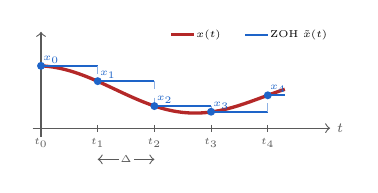
\begin{tikzpicture}[scale=0.72, every node/.style={scale=0.72}]
        % axes
        \draw[->, mambagray, thin] (-0.15, 0) -- (5.1, 0) node[right, font=\scriptsize] {$t$};
        \draw[->, mambagray, thin] (0, -0.15) -- (0, 1.7);
        % tick labels at t_0 ... t_4
        \foreach \i in {0,1,2,3,4} {
          \draw[mambagray, thin] (\i, 0.06) -- (\i, -0.06);
          \node[font=\tiny, mambagray, below] at (\i, -0.05) {$t_{\i}$};
        }
        % Delta brace between t_1 and t_2
        \draw[<->, mambagray, thin] (1, -0.55) -- (2, -0.55);
        \node[font=\tiny, mambagray, fill=white, inner sep=1pt] at (1.5, -0.55) {$\Delta$};

        % continuous x(t)
        \draw[mambared, very thick, smooth, samples=80, domain=0:4.3]
          plot (\x, {0.75 + 0.35*cos(1.2*\x r) - 0.05*\x});

        % ZOH staircase (sample values match x(t_k))
        \def\sA{1.10}  % t=0
        \def\sB{0.83}  % t=1
        \def\sC{0.39}  % t=2
        \def\sD{0.29}  % t=3
        \def\sE{0.58}  % t=4
        \draw[mambablue, thick] (0,\sA) -- (1,\sA);
        \draw[mambablue, thick] (1,\sB) -- (2,\sB);
        \draw[mambablue, thick] (2,\sC) -- (3,\sC);
        \draw[mambablue, thick] (3,\sD) -- (4,\sD);
        \draw[mambablue, thick] (4,\sE) -- (4.3,\sE);
        % vertical jumps (dashed)
        \draw[mambablue!50, dashed, thin] (1,\sA) -- (1,\sB);
        \draw[mambablue!50, dashed, thin] (2,\sB) -- (2,\sC);
        \draw[mambablue!50, dashed, thin] (3,\sC) -- (3,\sD);
        \draw[mambablue!50, dashed, thin] (4,\sD) -- (4,\sE);
        % sample dots
        \fill[mambablue] (0,\sA) circle (0.07);
        \fill[mambablue] (1,\sB) circle (0.07);
        \fill[mambablue] (2,\sC) circle (0.07);
        \fill[mambablue] (3,\sD) circle (0.07);
        \fill[mambablue] (4,\sE) circle (0.07);
        % sample labels above dots
        \node[font=\tiny, mambablue, above right, inner sep=1pt] at (0,\sA) {$x_0$};
        \node[font=\tiny, mambablue, above right, inner sep=1pt] at (1,\sB) {$x_1$};
        \node[font=\tiny, mambablue, above right, inner sep=1pt] at (2,\sC) {$x_2$};
        \node[font=\tiny, mambablue, above right, inner sep=1pt] at (3,\sD) {$x_3$};
        \node[font=\tiny, mambablue, above right, inner sep=1pt] at (4,\sE) {$x_4$};

        % legend
        \draw[mambared, very thick] (2.3,1.65) -- (2.7,1.65);
        \node[font=\tiny, right, inner sep=1pt] at (2.7,1.65) {$x(t)$};
        \draw[mambablue, thick] (3.6,1.65) -- (4.0,1.65);
        \node[font=\tiny, right, inner sep=1pt] at (4.0,1.65) {ZOH $\tilde{x}(t)$};
      \end{tikzpicture}
    \end{column}
  \end{columns}

  Then $x_k$ leaves the integral. Substitute $u = t_k + \Delta - s$ ($\mathrm{d}u = -\mathrm{d}s$, $u\colon \Delta \to 0$) and use the antiderivative $\bar{A}^{-1} e^{\bar{A} u}$ (valid for invertible $\bar{A}$, since $\tfrac{\mathrm{d}}{\mathrm{d}u}\bigl(\bar{A}^{-1} e^{\bar{A} u}\bigr) = e^{\bar{A} u}$):
  \[
    \int_{t_k}^{t_k+\Delta} e^{\bar{A}(t_k+\Delta-s)}\,\mathrm{d}s
    \;=\; \int_0^{\Delta} e^{\bar{A} u}\,\mathrm{d}u
    \;=\; \bigl[\bar{A}^{-1} e^{\bar{A} u}\bigr]_0^{\Delta}
    \;=\; \bar{A}^{-1}\bigl(e^{\bar{A}\Delta} - I\bigr).
  \]

  Writing $h_k := h(t_k)$, we obtain the \textbf{exact-under-ZOH discrete recurrence}
  \[
    h_{k+1} \;=\; \underbrace{e^{\bar{A}\Delta}}_{A}\, h_k
    \;+\; \underbrace{\bar{A}^{-1}\bigl(e^{\bar{A}\Delta} - I\bigr)\bar{B}}_{B}\, x_k,
    \qquad y_k = C\, h_k.
  \]

  \begin{itemize}
    \item The output $y(t) = C\,h(t)$ is already pointwise, so $C$ is unchanged.
    \item No truncation error from the integration itself; the only approximation is the staircase assumption on $x$.
    \item Smaller $\Delta$ $\Rightarrow$ ZOH is a better approximation of the true input; larger $\Delta$ $\Rightarrow$ fewer, coarser steps.
  \end{itemize}
\end{frame}

% -----------------------------------------------------------------------
\begin{frame}{The Discrete SSM Recurrence}

  With $A = e^{\bar{A}\Delta}$ and $B = \bar{A}^{-1}(e^{\bar{A}\Delta} - I)\bar{B}$, one step of the SSM reads:

  \begin{center}
  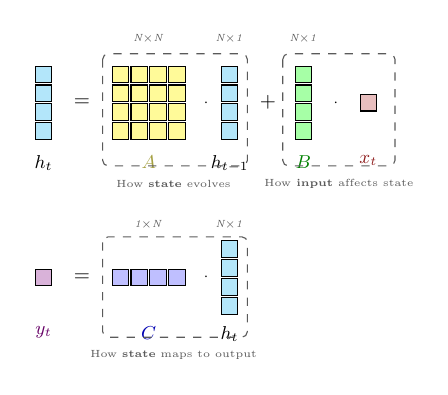
\begin{tikzpicture}[
    scale=0.75, every node/.style={scale=0.75},
    mat/.style={draw, thin, minimum size=0.28cm, inner sep=0pt},
  ]
    % === State equation: h_t = A * h_{t-1} + B * x_t ===
    % h_t vector (cyan, Nx1)
    \foreach \r in {0,...,3} {
      \node[mat, fill=cyan!30] at (0, -\r*0.32) {};
    }
    \node[font=\small\bfseries, below] at (0, -1.25) {$h_t$};

    \node[font=\normalsize] at (0.65, -0.48) {$=$};

    % A matrix (yellow, NxN)
    \foreach \r in {0,...,3} {
      \foreach \c in {0,...,3} {
        \node[mat, fill=yellow!40] at (1.3+\c*0.32, -\r*0.32) {};
      }
    }
    \node[font=\small\bfseries, below, yellow!60!black] at (1.78, -1.25) {$A$};

    \node[font=\scriptsize] at (2.75, -0.48) {$\cdot$};

    % h_{t-1} vector (cyan, Nx1)
    \foreach \r in {0,...,3} {
      \node[mat, fill=cyan!30] at (3.15, -\r*0.32) {};
    }
    \node[font=\small\bfseries, below] at (3.15, -1.25) {$h_{t-1}$};

    \node[font=\normalsize] at (3.8, -0.48) {$+$};

    % B vector (green, Nx1)
    \foreach \r in {0,...,3} {
      \node[mat, fill=green!35] at (4.4, -\r*0.32) {};
    }
    \node[font=\small\bfseries, below, green!50!black] at (4.4, -1.25) {$B$};

    \node[font=\scriptsize] at (4.95, -0.48) {$\cdot$};

    % x_t as a single scalar block
    \node[mat, fill=mambared!30] at (5.5, -0.48) {};
    \node[font=\small\bfseries, below, mambared!80!black] at (5.5, -1.25) {$x_t$};

    % --- dashed grouping boxes with annotations ---
    \draw[dashed, mambagray, rounded corners=2pt] (1.0,0.35) rectangle (3.45,-1.55);
    \node[font=\tiny, mambagray, align=center] at (2.2, -1.85) {How \textbf{state} evolves};
    \draw[dashed, mambagray, rounded corners=2pt] (4.05,0.35) rectangle (5.95,-1.55);
    \node[font=\tiny, mambagray, align=center] at (5.0, -1.85) {How \textbf{input} affects state};

    % === Output equation: y_t = C * h_t ===
    \def\offy{-3.3}

    % y_t as a single scalar block
    \node[mat, fill=violet!30] at (0, \offy-0.14) {};
    \node[font=\small\bfseries, below, violet!80!black] at (0, \offy-0.85) {$y_t$};

    \node[font=\normalsize] at (0.65, \offy-0.14) {$=$};

    % C vector (blue, 1xN)
    \foreach \c in {0,...,3} {
      \node[mat, fill=blue!25] at (1.3+\c*0.32, \offy-0.14) {};
    }
    \node[font=\small\bfseries, below, blue!70!black] at (1.78, \offy-0.85) {$C$};

    \node[font=\scriptsize] at (2.75, \offy-0.14) {$\cdot$};

    % h_t vector (cyan, Nx1)
    \foreach \r in {0,...,3} {
      \node[mat, fill=cyan!30] at (3.15, \offy-0.14+0.48-\r*0.32) {};
    }
    \node[font=\small\bfseries, below] at (3.15, \offy-0.85) {$h_t$};

    % --- dashed grouping ---
    \draw[dashed, mambagray, rounded corners=2pt] (1.0,\offy+0.55) rectangle (3.45,\offy-1.15);
    \node[font=\tiny, mambagray, align=center] at (2.2, \offy-1.45) {How \textbf{state} maps to output};

    % Dimension annotations
    \node[font=\tiny, mambagray] at (1.78, 0.6) {\textit{N$\times$N}};
    \node[font=\tiny, mambagray] at (3.15, 0.6) {\textit{N$\times$1}};
    \node[font=\tiny, mambagray] at (4.4, 0.6) {\textit{N$\times$1}};
    \node[font=\tiny, mambagray] at (1.78, \offy+0.75) {\textit{1$\times$N}};
    \node[font=\tiny, mambagray] at (3.15, \offy+0.75) {\textit{N$\times$1}};
  \end{tikzpicture}
  \end{center}

  \begin{itemize}
    \item Looks like a linear RNN, but with structured matrices $A, B, C$.
    \item The step size $\Delta$ is the discretization granularity: how much continuous time each step represents.
    \item $\Delta$ will take on a richer, \emph{gating-like} role once we make it input-dependent in selective SSMs (Mamba).
  \end{itemize}
\end{frame}

% -----------------------------------------------------------------------
\begin{frame}{Unrolling the Recurrence $\Rightarrow$ Convolution}

  Assume $h_{-1} = 0$ and LTI ($A, B, C$ constant). Expand step by step:
  \begin{align*}
    h_0 &= B\,x_0
      & y_0 &= C\,h_0 &&= C B\,x_0 \\
    h_1 &= A\,h_0 + B\,x_1 = A B\,x_0 + B\,x_1
      & y_1 &= C\,h_1 &&= C A B\,x_0 + C B\,x_1 \\
    h_2 &= A\,h_1 + B\,x_2 = A^2 B\,x_0 + A B\,x_1 + B\,x_2
      & y_2 &= C\,h_2 &&= C A^2 B\,x_0 + C A B\,x_1 + C B\,x_2 \\
    &\ \vdots & &\ \vdots
  \end{align*}

  The pattern continues. At step $t$:
  \[
    y_t \;=\; C A^t B\, x_0 + C A^{t-1} B\, x_1 + \cdots + C B\, x_t
    \;=\; \sum_{k=0}^{t} \underbrace{C A^k B}_{\bar{K}_k}\, x_{t-k}.
  \]

  \begin{itemize}
    \item This is a \textbf{causal convolution} $y = \bar{K} \ast x$ with kernel $\bar{K} = (C B,\, C A B,\, C A^2 B,\, \ldots,\, C A^{T-1} B)$.
    \item Each output $y_t$ only sees past inputs $x_0, \ldots, x_t$ (causal), weighted by $\bar{K}_k$.
  \end{itemize}
\end{frame}

% -----------------------------------------------------------------------
\begin{frame}{The Dual View: Recurrence vs.\ Convolution}

  Same model, two computational modes:
  \begin{columns}
    \begin{column}{0.48\textwidth}
      \textbf{Recurrent mode}
      \begin{itemize}
        \item Apply $h_t = A h_{t-1} + B x_t$, $y_t = C h_t$ step by step
        \item $O(N)$ per step, $O(N)$ memory
        \item Sequential $\Rightarrow$ good for autoregressive inference
      \end{itemize}
    \end{column}
    \begin{column}{0.48\textwidth}
      \textbf{Convolutional mode}
      \begin{itemize}
        \item Precompute kernel $\bar{K}$, apply $y = \bar{K} \ast x$ via FFT
        \item $O(T \log T)$ in $T$, parallel over time
        \item Good for training on long sequences
      \end{itemize}
    \end{column}
  \end{columns}

  \vspace{0.5em}
  \begin{block}{S4~\cite{gu2022s4}}
    Structured State Spaces for Sequences (S4) uses HiPPO initialization and diagonal structure for $\bar{A}$ to make the kernel $\bar{K}$ computable in $O(T)$. First SSM to match Transformers on long-range benchmarks.
  \end{block}
\end{frame}

% -----------------------------------------------------------------------
\begin{frame}{The Limitation of LTI Models}

  LTI SSMs apply the \emph{same} convolution kernel to every input, regardless of content.

  \vspace{0.5em}
  \textbf{Example:} Consider the task of selectively copying tokens from context.

  \begin{center}
    \begin{tikzpicture}[
      tok/.style={minimum width=0.65cm, minimum height=0.55cm, draw, font=\small, inner sep=1pt},
    ]
      \node[tok, fill=mambablue!20] at (0,0) {A};
      \node[tok] at (0.7,0) {x};
      \node[tok] at (1.4,0) {x};
      \node[tok, fill=mambared!20] at (2.1,0) {B};
      \node[tok] at (2.8,0) {x};
      \node[tok, fill=mambagreen!20] at (3.5,0) {C};
      \node[tok] at (4.2,0) {x};
      \node[tok] at (4.9,0) {x};

      \draw[-Stealth, thick] (5.4,0) -- (6.0,0);

      \node[tok, fill=mambablue!20] at (6.5,0) {A};
      \node[tok, fill=mambared!20] at (7.2,0) {B};
      \node[tok, fill=mambagreen!20] at (7.9,0) {C};
    \end{tikzpicture}
  \end{center}

  \begin{itemize}
    \item An LTI model treats every token identically. It cannot \emph{selectively} remember some tokens and ignore others based on content
    \item A fixed kernel is fundamentally \alert{content-agnostic}
    \item Transformers solve this via content-dependent attention weights
  \end{itemize}

  \vspace{0.3em}
  \begin{alertblock}{Insight}
    To make SSMs truly powerful, the parameters must be \textbf{input-dependent}. This enables \emph{selectivity} but \alert{breaks LTI} and with it the convolutional / FFT mode that made parallel training cheap.
  \end{alertblock}

  \textbf{The central design tension} for the rest of this section:
  \begin{itemize}
    \item \textbf{Keep} content-dependent selectivity (needed for modeling power).
    \item \textbf{Recover} sequence-parallel training (so we can train on long contexts).
  \end{itemize}

  \textbf{What comes next:}
  \begin{itemize}
    \item \textbf{Mamba 1:} solves this at the hardware level — a \emph{selective scan} fused into one GPU kernel that keeps the state in SRAM, so the sequential recurrence runs fast enough in practice.
    \item \textbf{Mamba 2:} restricts $\bar{A}$ to scalar $\times$ identity (State Space Duality), which re-exposes a matmul-friendly, parallel training algorithm while retaining input-dependent $B_t, C_t, \Delta_t$.
  \end{itemize}
\end{frame}

% =======================================================================
\subsubsection{Mamba: Selective State Spaces}

% -----------------------------------------------------------------------
\begin{frame}{Selectivity: The Core Idea of Mamba~\cite{gu2024mamba}}

  \textbf{Mamba} makes the SSM parameters \emph{functions of the input}:
  \[
    B_t = \text{Linear}_B(x_t), \quad C_t = \text{Linear}_C(x_t), \quad \Delta_t = \text{softplus}(\text{Linear}_\Delta(x_t)).
  \]
  The discrete recurrence becomes \textbf{time-varying}:
  \[
    \boxed{h_t = A_t\, h_{t-1} + B_t\, x_t, \qquad y_t = C_t^\top h_t}
    \qquad \text{with } A_t = \exp(\Delta_t\, \bar{A}).
  \]
  Only $B_t, C_t, \Delta_t$ are input-dependent; $\bar{A}$ is a fixed, learned structural prior.

  \vspace{0.3em}
  \textbf{Structure of $\bar{A}$:}

  \begin{columns}[T]
    \begin{column}{0.5\textwidth}
      \textbf{Mamba 1}: $\bar{A}$ is \emph{diagonal} (S4D-style)
      \[
        \bar{A} = \operatorname{diag}(-a_1,\, -a_2,\, \ldots,\, -a_N),\ a_i > 0
      \]
      \begin{itemize}
        \item $N$ independent decay rates per channel, HiPPO/S4D-initialized
        \item $A_t = \operatorname{diag}\!\bigl(e^{-a_i \Delta_t}\bigr)$ stays diagonal
        \item Each hidden dimension decays at its own rate $\Rightarrow$ multi-timescale memory
      \end{itemize}
    \end{column}
    \begin{column}{0.5\textwidth}
      \textbf{Mamba 2}: $\bar{A}$ is \emph{scalar $\times$ identity}
      \[
        \bar{A} = -a\, I_N,\qquad a > 0
      \]
      \begin{itemize}
        \item A single learned decay rate shared across all $N$ state channels
        \item $A_t = e^{-a \Delta_t}\, I_N \eqqcolon \alpha_t\, I_N$ with $\alpha_t \in (0,1)$
        \item Stricter prior, but this scalar-structured $A_t$ is what unlocks the State Space Duality with linear attention (next section)
      \end{itemize}
    \end{column}
  \end{columns}
\end{frame}

% -----------------------------------------------------------------------
\begin{frame}{$\Delta_t$ as an Input-Dependent Gate}

  \begin{itemize}
    \item $\Delta_t$: second input-dependent parameter governing selectivity.
    \item Recurrence:
      \[
        h_t \;=\; \underbrace{A_t}_{\text{state retention}}\, h_{t-1} \;+\; \underbrace{B_t}_{\text{input injection}}\, x_t
      \]
    \item Both coefficients determined by $\Delta_t$ via the zero-order hold:
      \[
        A_t = e^{\bar{A}\Delta_t}, \qquad B_t = \bar{A}^{-1}\bigl(e^{\bar{A}\Delta_t} - I\bigr)\bar{B}.
      \]
    \item Both depend on the \emph{same} scalar $\Delta_t$ (per channel).
  \end{itemize}

  Two asymptotic regimes:

  \begin{itemize}
    \item \textbf{$\Delta_t \to 0$:}
      \begin{itemize}
        \item $A_t \approx I$ \hfill (state preserved)
        \item $B_t \approx \Delta_t\,\bar{B} \to 0$ \hfill (input suppressed)
        \item $\Rightarrow h_t \approx h_{t-1}$: state propagated unchanged, $x_t$ negligible.
      \end{itemize}
    \item \textbf{$\Delta_t \to \infty$:}
      \begin{itemize}
        \item $A_t \to 0$ \hfill (state attenuated)
        \item $B_t \to -\bar{A}^{-1}\bar{B}$ \hfill (input fully integrated)
        \item $\Rightarrow h_t \approx -\bar{A}^{-1}\bar{B}\, x_t$: prior state overwritten, $h_t$ depends only on $x_t$.
      \end{itemize}
    \item $\Delta_t$ thus acts as a learned, input-dependent \textbf{write/forget gate} controlling the contribution of $x_t$ to the latent state: the selection mechanism.
  \end{itemize}
\end{frame}

% -----------------------------------------------------------------------
\begin{frame}{The Parallel Scan}

  \begin{itemize}
    \item Input-dependent parameters preclude the convolutional mode. Evaluate
      \[
        h_t = A_t\, h_{t-1} + B_t\, x_t, \qquad t = 0, \ldots, T{-}1.
      \]
    \item Naive evaluation: sequential, $T$ steps.
    \item Key observations:
      \begin{itemize}
        \item Each step is an \textbf{affine map} $h \mapsto A_t h + b_t$ with $b_t = B_t x_t$.
        \item Composition of affine maps is affine and \textbf{associative}.
        \item Associative operations admit a \textbf{parallel prefix scan} (generalised prefix-sum).
      \end{itemize}
    \item Complexity:
      \begin{center}
        \begin{tabular}{lcc}
          \toprule
          & \textbf{Sequential (RNN)} & \textbf{Parallel scan} \\
          \midrule
          Depth      & $T$    & $O(\log T)$ \\
          Total work & $O(T)$ & $O(T)$--$O(T\log T)$ \\
          \bottomrule
        \end{tabular}
      \end{center}
    \item Loss of the convolutional mode does not entail sequential inference.
  \end{itemize}
\end{frame}

% -----------------------------------------------------------------------
\begin{frame}{Parallel Prefix Sum (Hillis-Steele Scan)}

  \textbf{Problem}: given $(x_1,\ldots,x_8)$, compute all prefix sums $s_t = \sum_{k=1}^{t} x_k$ in parallel.

  \textbf{Idea}: at each step, every element adds the element \emph{stride} positions to its left. After $\lceil\log_2 T\rceil$ steps every prefix is complete. We write $x_{i:j} := \sum_{k=i}^{j} x_k$.

  \begin{center}
  \begin{tikzpicture}[
    cell/.style={minimum width=1.0cm, minimum height=0.48cm, draw, rounded corners=1pt,
                 font=\tiny, inner sep=1pt},
    combine/.style={-Stealth, semithick},
    scale=0.85, every node/.style={scale=0.85},
  ]
    \def\dy{-1.35}
    \def\dx{1.25}

    % ---------- Row 0: input ----------
    \node[cell, fill=mambared!15] (a0) at (0*\dx, 0) {$x_1$};
    \node[cell, fill=mambared!15] (a1) at (1*\dx, 0) {$x_2$};
    \node[cell, fill=mambared!15] (a2) at (2*\dx, 0) {$x_3$};
    \node[cell, fill=mambared!15] (a3) at (3*\dx, 0) {$x_4$};
    \node[cell, fill=mambared!15] (a4) at (4*\dx, 0) {$x_5$};
    \node[cell, fill=mambared!15] (a5) at (5*\dx, 0) {$x_6$};
    \node[cell, fill=mambared!15] (a6) at (6*\dx, 0) {$x_7$};
    \node[cell, fill=mambared!15] (a7) at (7*\dx, 0) {$x_8$};
    \node[font=\scriptsize, anchor=east] at (-0.6, 0) {Input};

    % ---------- Row 1: stride 1 ----------
    \node[cell, fill=yellow!25] (b0) at (0*\dx, \dy) {$x_1$};
    \node[cell, fill=yellow!25] (b1) at (1*\dx, \dy) {$x_{1:2}$};
    \node[cell, fill=yellow!25] (b2) at (2*\dx, \dy) {$x_{2:3}$};
    \node[cell, fill=yellow!25] (b3) at (3*\dx, \dy) {$x_{3:4}$};
    \node[cell, fill=yellow!25] (b4) at (4*\dx, \dy) {$x_{4:5}$};
    \node[cell, fill=yellow!25] (b5) at (5*\dx, \dy) {$x_{5:6}$};
    \node[cell, fill=yellow!25] (b6) at (6*\dx, \dy) {$x_{6:7}$};
    \node[cell, fill=yellow!25] (b7) at (7*\dx, \dy) {$x_{7:8}$};
    \node[font=\scriptsize, anchor=east] at (-0.6, \dy) {Step 1};
    \node[font=\tiny, mambagray, anchor=west] at (7*\dx+0.65, \dy) {stride $1$};
    \foreach \i in {1,...,7} {
      \pgfmathtruncatemacro{\j}{\i-1}
      \draw[combine, mambagreen!80!black] (a\j.south) -- (b\i.north);
    }

    % ---------- Row 2: stride 2 ----------
    \node[cell, fill=yellow!40] (c0) at (0*\dx, 2*\dy) {$x_1$};
    \node[cell, fill=yellow!40] (c1) at (1*\dx, 2*\dy) {$x_{1:2}$};
    \node[cell, fill=yellow!40] (c2) at (2*\dx, 2*\dy) {$x_{1:3}$};
    \node[cell, fill=yellow!40] (c3) at (3*\dx, 2*\dy) {$x_{1:4}$};
    \node[cell, fill=yellow!40] (c4) at (4*\dx, 2*\dy) {$x_{2:5}$};
    \node[cell, fill=yellow!40] (c5) at (5*\dx, 2*\dy) {$x_{3:6}$};
    \node[cell, fill=yellow!40] (c6) at (6*\dx, 2*\dy) {$x_{4:7}$};
    \node[cell, fill=yellow!40] (c7) at (7*\dx, 2*\dy) {$x_{5:8}$};
    \node[font=\scriptsize, anchor=east] at (-0.6, 2*\dy) {Step 2};
    \node[font=\tiny, mambagray, anchor=west] at (7*\dx+0.65, 2*\dy) {stride $2$};
    \foreach \i in {2,...,7} {
      \pgfmathtruncatemacro{\j}{\i-2}
      \draw[combine, mambablue!80!black] (b\j.south) -- (c\i.north);
    }

    % ---------- Row 3: stride 4 (result = all prefixes from x_1) ----------
    \node[cell, fill=mambagreen!25] (d0) at (0*\dx, 3*\dy) {$x_1$};
    \node[cell, fill=mambagreen!25] (d1) at (1*\dx, 3*\dy) {$x_{1:2}$};
    \node[cell, fill=mambagreen!25] (d2) at (2*\dx, 3*\dy) {$x_{1:3}$};
    \node[cell, fill=mambagreen!25] (d3) at (3*\dx, 3*\dy) {$x_{1:4}$};
    \node[cell, fill=mambagreen!25] (d4) at (4*\dx, 3*\dy) {$x_{1:5}$};
    \node[cell, fill=mambagreen!25] (d5) at (5*\dx, 3*\dy) {$x_{1:6}$};
    \node[cell, fill=mambagreen!25] (d6) at (6*\dx, 3*\dy) {$x_{1:7}$};
    \node[cell, fill=mambagreen!25] (d7) at (7*\dx, 3*\dy) {$x_{1:8}$};
    \node[font=\scriptsize, anchor=east] at (-0.6, 3*\dy) {Result};
    \node[font=\tiny, mambagray, anchor=west] at (7*\dx+0.65, 3*\dy) {stride $4$};
    \foreach \i in {4,...,7} {
      \pgfmathtruncatemacro{\j}{\i-4}
      \draw[combine, violet!80!black] (c\j.south) -- (d\i.north);
    }

    % ---------- legend ----------
    \draw[combine, mambagreen!80!black] (0.3, 3*\dy-0.75) -- ++(0.5,0)
      node[right, font=\tiny, black] {combine from stride 1};
    \draw[combine, mambablue!80!black] (3.2, 3*\dy-0.75) -- ++(0.5,0)
      node[right, font=\tiny, black] {combine from stride 2};
    \draw[combine, violet!80!black] (6.1, 3*\dy-0.75) -- ++(0.5,0)
      node[right, font=\tiny, black] {combine from stride 4};
  \end{tikzpicture}
  \end{center}

  \begin{itemize}
    \item Cells without an incoming arrow pass through unchanged.
    \item $\lceil\log_2 T\rceil$ parallel steps $\Rightarrow$ depth $O(\log T)$, work $O(T\log T)$.
    \item Here we use $+$ for illustration. The same algorithm works for \emph{any} associative operator $\oplus$, as we will see next.
  \end{itemize}
\end{frame}

% -----------------------------------------------------------------------
\begin{frame}{Blelloch Scan: Up-Sweep (Reduce)}

  \begin{itemize}
    \item Hillis-Steele does $O(T\log T)$ total work. The \textbf{Blelloch scan} reduces this to $O(T)$ using two phases.
    \item \textbf{Phase 1 (up-sweep)}: at each level, only positions at stride $2^{d+1}$ accumulate from their left neighbor at distance $2^d$.
  \end{itemize}

  \begin{center}
  \begin{tikzpicture}[
    cell/.style={minimum width=1.0cm, minimum height=0.48cm, draw, rounded corners=1pt,
                 font=\tiny, inner sep=1pt},
    gray cell/.style={cell, fill=gray!12, text=gray!50},
    combine/.style={-Stealth, semithick},
    scale=0.85, every node/.style={scale=0.85},
  ]
    \def\dy{-1.35}
    \def\dx{1.25}

    % ---------- Row 0: input ----------
    \node[cell, fill=mambared!15] (a0) at (0*\dx, 0) {$x_1$};
    \node[cell, fill=mambared!15] (a1) at (1*\dx, 0) {$x_2$};
    \node[cell, fill=mambared!15] (a2) at (2*\dx, 0) {$x_3$};
    \node[cell, fill=mambared!15] (a3) at (3*\dx, 0) {$x_4$};
    \node[cell, fill=mambared!15] (a4) at (4*\dx, 0) {$x_5$};
    \node[cell, fill=mambared!15] (a5) at (5*\dx, 0) {$x_6$};
    \node[cell, fill=mambared!15] (a6) at (6*\dx, 0) {$x_7$};
    \node[cell, fill=mambared!15] (a7) at (7*\dx, 0) {$x_8$};
    \node[font=\scriptsize, anchor=east] at (-0.6, 0) {Input};

    % ---------- Row 1: stride 1 (positions 1,3,5,7 active) ----------
    \node[gray cell] (b0) at (0*\dx, \dy) {$x_1$};
    \node[cell, fill=yellow!25] (b1) at (1*\dx, \dy) {$x_{1:2}$};
    \node[gray cell] (b2) at (2*\dx, \dy) {$x_3$};
    \node[cell, fill=yellow!25] (b3) at (3*\dx, \dy) {$x_{3:4}$};
    \node[gray cell] (b4) at (4*\dx, \dy) {$x_5$};
    \node[cell, fill=yellow!25] (b5) at (5*\dx, \dy) {$x_{5:6}$};
    \node[gray cell] (b6) at (6*\dx, \dy) {$x_7$};
    \node[cell, fill=yellow!25] (b7) at (7*\dx, \dy) {$x_{7:8}$};
    \node[font=\scriptsize, anchor=east] at (-0.6, \dy) {Level 1};
    \node[font=\tiny, mambagray, anchor=west] at (7*\dx+0.65, \dy) {stride $1$};
    % arrows: each active position accumulates from its left neighbor
    \foreach \src/\dst in {0/1, 2/3, 4/5, 6/7} {
      \draw[combine, mambagreen!80!black] (a\src.south) -- (b\dst.north);
    }

    % ---------- Row 2: stride 2 (positions 3,7 active) ----------
    \node[gray cell] (c0) at (0*\dx, 2*\dy) {$x_1$};
    \node[gray cell] (c1) at (1*\dx, 2*\dy) {$x_{1:2}$};
    \node[gray cell] (c2) at (2*\dx, 2*\dy) {$x_3$};
    \node[cell, fill=yellow!40] (c3) at (3*\dx, 2*\dy) {$x_{1:4}$};
    \node[gray cell] (c4) at (4*\dx, 2*\dy) {$x_5$};
    \node[gray cell] (c5) at (5*\dx, 2*\dy) {$x_{5:6}$};
    \node[gray cell] (c6) at (6*\dx, 2*\dy) {$x_7$};
    \node[cell, fill=yellow!40] (c7) at (7*\dx, 2*\dy) {$x_{5:8}$};
    \node[font=\scriptsize, anchor=east] at (-0.6, 2*\dy) {Level 2};
    \node[font=\tiny, mambagray, anchor=west] at (7*\dx+0.65, 2*\dy) {stride $2$};
    \draw[combine, mambablue!80!black] (b1.south) -- (c3.north);
    \draw[combine, mambablue!80!black] (b5.south) -- (c7.north);

    % ---------- Row 3: stride 4 (position 7 active = root) ----------
    \node[gray cell] (d0) at (0*\dx, 3*\dy) {$x_1$};
    \node[gray cell] (d1) at (1*\dx, 3*\dy) {$x_{1:2}$};
    \node[gray cell] (d2) at (2*\dx, 3*\dy) {$x_3$};
    \node[gray cell] (d3) at (3*\dx, 3*\dy) {$x_{1:4}$};
    \node[gray cell] (d4) at (4*\dx, 3*\dy) {$x_5$};
    \node[gray cell] (d5) at (5*\dx, 3*\dy) {$x_{5:6}$};
    \node[gray cell] (d6) at (6*\dx, 3*\dy) {$x_7$};
    \node[cell, fill=mambagreen!25] (d7) at (7*\dx, 3*\dy) {$x_{1:8}$};
    \node[font=\scriptsize, anchor=east] at (-0.6, 3*\dy) {Root};
    \node[font=\tiny, mambagray, anchor=west] at (7*\dx+0.65, 3*\dy) {stride $4$};
    \draw[combine, violet!80!black] (c3.south) -- (d7.north);
  \end{tikzpicture}
  \end{center}

  \begin{itemize}
    \item Only the colored cells participate at each level; gray cells are untouched.
    \item Total additions: $4 + 2 + 1 = T{-}1$.
    \item After up-sweep, every position $2^k$ holds the prefix sum $x_{1:2^k}$ (here positions $2, 4, 8$); the remaining positions still hold partial subtree sums. The down-sweep fills in all other prefixes.
  \end{itemize}
\end{frame}

% -----------------------------------------------------------------------
\begin{frame}{Blelloch Scan: Down-Sweep}

  \begin{itemize}
    \item \textbf{Phase 2 (down-sweep)}: propagate top-down. Set root to $0$; at each level, left $\gets$ parent, right $\gets$ parent $+$ old left.
  \end{itemize}

  \begin{center}
  \begin{tikzpicture}[
    cell/.style={minimum width=1.0cm, minimum height=0.48cm, draw, rounded corners=1pt,
                 font=\tiny, inner sep=1pt},
    gray cell/.style={cell, fill=gray!12, text=gray!45},
    parent/.style={-Stealth, semithick, mambablue!80!black},
    oldleft/.style={-Stealth, semithick, mambared!70!black},
    scale=0.85, every node/.style={scale=0.85},
  ]
    \def\dy{-1.35}
    \def\dx{1.25}

    % ---------- Row 0: up-sweep result with root zeroed ----------
    % Gray cells show carried up-sweep values; pos 7 is zeroed (blue)
    \node[gray cell] (a0) at (0*\dx, 0) {$x_1$};
    \node[gray cell] (a1) at (1*\dx, 0) {$x_{1:2}$};
    \node[gray cell] (a2) at (2*\dx, 0) {$x_3$};
    \node[gray cell] (a3) at (3*\dx, 0) {$x_{1:4}$};
    \node[gray cell] (a4) at (4*\dx, 0) {$x_5$};
    \node[gray cell] (a5) at (5*\dx, 0) {$x_{5:6}$};
    \node[gray cell] (a6) at (6*\dx, 0) {$x_7$};
    \node[cell, fill=mambablue!20] (a7) at (7*\dx, 0) {$0$};
    \node[font=\scriptsize, anchor=east] at (-0.6, 0) {Start};

    % ---------- Row 1: stride 4 (positions 3,7 active) ----------
    \node[gray cell] (b0) at (0*\dx, \dy) {$x_1$};
    \node[gray cell] (b1) at (1*\dx, \dy) {$x_{1:2}$};
    \node[gray cell] (b2) at (2*\dx, \dy) {$x_3$};
    \node[cell, fill=mambablue!20] (b3) at (3*\dx, \dy) {$0$};
    \node[gray cell] (b4) at (4*\dx, \dy) {$x_5$};
    \node[gray cell] (b5) at (5*\dx, \dy) {$x_{5:6}$};
    \node[gray cell] (b6) at (6*\dx, \dy) {$x_7$};
    \node[cell, fill=mambablue!20] (b7) at (7*\dx, \dy) {$x_{1:4}$};
    \node[font=\scriptsize, anchor=east] at (-0.6, \dy) {Level 1};
    \node[font=\tiny, mambagray, anchor=west] at (7*\dx+0.65, \dy) {stride $4$};
    % parent (right pos) propagates to left child
    \draw[parent] (a7.south) -- (b3.north);
    % right child = parent + old left
    \draw[parent] (a7.south) -- (b7.north);
    \draw[oldleft] (a3.south) -- (b7.north);

    % ---------- Row 2: stride 2 (positions 1,3,5,7 active) ----------
    \node[gray cell] (c0) at (0*\dx, 2*\dy) {$x_1$};
    \node[cell, fill=mambablue!20] (c1) at (1*\dx, 2*\dy) {$0$};
    \node[gray cell] (c2) at (2*\dx, 2*\dy) {$x_3$};
    \node[cell, fill=mambablue!20] (c3) at (3*\dx, 2*\dy) {$x_{1:2}$};
    \node[gray cell] (c4) at (4*\dx, 2*\dy) {$x_5$};
    \node[cell, fill=mambablue!20] (c5) at (5*\dx, 2*\dy) {$x_{1:4}$};
    \node[gray cell] (c6) at (6*\dx, 2*\dy) {$x_7$};
    \node[cell, fill=mambablue!20] (c7) at (7*\dx, 2*\dy) {$x_{1:6}$};
    \node[font=\scriptsize, anchor=east] at (-0.6, 2*\dy) {Level 2};
    \node[font=\tiny, mambagray, anchor=west] at (7*\dx+0.65, 2*\dy) {stride $2$};
    % parent to left
    \draw[parent] (b3.south) -- (c1.north);
    \draw[parent] (b7.south) -- (c5.north);
    % right = parent + old left
    \draw[parent] (b3.south) -- (c3.north);
    \draw[oldleft] (b1.south) -- (c3.north);
    \draw[parent] (b7.south) -- (c7.north);
    \draw[oldleft] (b5.south) -- (c7.north);

    % ---------- Row 3: stride 1 (all positions active = result) ----------
    \node[cell, fill=mambagreen!20] (d0) at (0*\dx, 3*\dy) {$0$};
    \node[cell, fill=mambagreen!20] (d1) at (1*\dx, 3*\dy) {$x_1$};
    \node[cell, fill=mambagreen!20] (d2) at (2*\dx, 3*\dy) {$x_{1:2}$};
    \node[cell, fill=mambagreen!20] (d3) at (3*\dx, 3*\dy) {$x_{1:3}$};
    \node[cell, fill=mambagreen!20] (d4) at (4*\dx, 3*\dy) {$x_{1:4}$};
    \node[cell, fill=mambagreen!20] (d5) at (5*\dx, 3*\dy) {$x_{1:5}$};
    \node[cell, fill=mambagreen!20] (d6) at (6*\dx, 3*\dy) {$x_{1:6}$};
    \node[cell, fill=mambagreen!20] (d7) at (7*\dx, 3*\dy) {$x_{1:7}$};
    \node[font=\scriptsize, anchor=east] at (-0.6, 3*\dy) {Result};
    \node[font=\tiny, mambagray, anchor=west] at (7*\dx+0.65, 3*\dy) {stride $1$};
    % parent to left
    \foreach \src in {1,3,5,7} {
      \pgfmathtruncatemacro{\dst}{\src-1}
      \draw[parent] (c\src.south) -- (d\dst.north);
    }
    % right = parent + old left
    \foreach \src in {1,3,5,7} {
      \pgfmathtruncatemacro{\oleft}{\src-1}
      \draw[parent] (c\src.south) -- (d\src.north);
      \draw[oldleft] (c\oleft.south) -- (d\src.north);
    }

    % ---------- legend ----------
    \draw[parent] (0.3, 3*\dy-0.75) -- ++(0.5,0)
      node[right, font=\tiny, black] {parent $\to$ child};
    \draw[oldleft] (4.0, 3*\dy-0.75) -- ++(0.5,0)
      node[right, font=\tiny, black] {old left $\to$ right child};
  \end{tikzpicture}
  \end{center}

  \begin{itemize}
    \item Leaves hold \textbf{exclusive prefix sums} ($\sum_{k<i} x_k$); add $x_i$ for inclusive.
    \item Both phases: $2(T{-}1) = O(T)$ work, $2\log_2 T$ depth.
  \end{itemize}

  \begin{center}
    \begin{tabular}{lcc}
      \toprule
      & \textbf{Hillis-Steele} & \textbf{Blelloch} \\
      \midrule
      Total work & $O(T\log T)$ & $O(T)$ \\
      Depth      & $\log_2 T$ & $2\log_2 T$ \\
      \bottomrule
    \end{tabular}
  \end{center}
\end{frame}

% -----------------------------------------------------------------------
\begin{frame}{Applying the Parallel Scan to the SSM}

  \begin{itemize}
    \item Map each time step to a pair $e_t = (A_t,\, b_t)$ with $b_t = B_t x_t$.
    \item Apply the scan under
    \(
      (A',\, b') \oplus (A,\, b) = (A'\!A,\ A'\!b + b').
    \)
  \end{itemize}

  \begin{center}
  \begin{tikzpicture}[
    cell/.style={minimum width=1.3cm, minimum height=0.5cm, draw, rounded corners=2pt,
                 font=\tiny, inner sep=2pt, align=center},
    combine/.style={-Stealth, semithick},
    scale=0.85, every node/.style={scale=0.85},
  ]
    \def\dy{-1.4}
    \def\dx{2.1}

    % ---------- Row 0: input pairs ----------
    \node[cell, fill=mambared!15] (a0) at (0*\dx, 0) {$e_0 = (A_0, b_0)$};
    \node[cell, fill=mambared!15] (a1) at (1*\dx, 0) {$e_1 = (A_1, b_1)$};
    \node[cell, fill=mambared!15] (a2) at (2*\dx, 0) {$e_2 = (A_2, b_2)$};
    \node[cell, fill=mambared!15] (a3) at (3*\dx, 0) {$e_3 = (A_3, b_3)$};
    \node[font=\scriptsize, anchor=east] at (-1.1, 0) {Input};

    % ---------- Row 1: after stride 1 ----------
    \node[cell, fill=yellow!25] (b0) at (0*\dx, \dy) {$e_0$};
    \node[cell, fill=yellow!25] (b1) at (1*\dx, \dy) {$e_{0:1}$};
    \node[cell, fill=yellow!25] (b2) at (2*\dx, \dy) {$e_{1:2}$};
    \node[cell, fill=yellow!25] (b3) at (3*\dx, \dy) {$e_{2:3}$};
    \node[font=\scriptsize, anchor=east] at (-1.1, \dy) {Step 1};
    \node[font=\tiny, mambagray, anchor=west] at (3*\dx+0.8, \dy) {stride $1$};
    \foreach \i in {1,...,3} {
      \pgfmathtruncatemacro{\j}{\i-1}
      \draw[combine, mambagreen!80!black] (a\j.south) -- (b\i.north);
    }

    % ---------- Row 2: after stride 2 (= result for T=4) ----------
    \node[cell, fill=mambagreen!20] (c0) at (0*\dx, 2*\dy) {$e_0$};
    \node[cell, fill=mambagreen!20] (c1) at (1*\dx, 2*\dy) {$e_{0:1}$};
    \node[cell, fill=mambagreen!20] (c2) at (2*\dx, 2*\dy) {$e_{0:2}$};
    \node[cell, fill=mambagreen!20] (c3) at (3*\dx, 2*\dy) {$e_{0:3}$};
    \node[font=\scriptsize, anchor=east] at (-1.1, 2*\dy) {Result};
    \node[font=\tiny, mambagray, anchor=west] at (3*\dx+0.8, 2*\dy) {stride $2$};
    \foreach \i in {2,3} {
      \pgfmathtruncatemacro{\j}{\i-2}
      \draw[combine, mambablue!80!black] (b\j.south) -- (c\i.north);
    }
  \end{tikzpicture}
  \end{center}

  \begin{itemize}
    \item \textbf{Reading off $h_t$:} the second component of $e_{0:t}$ (applied to $h_{-1}=0$) gives $h_t$.
    \item Example for position 2:
  \end{itemize}
  \[
    e_{0:2} = \underbrace{e_{1:2}}_{\text{step 1, pos 2}} \!\oplus\, \underbrace{e_0}_{\text{step 1, pos 0}}
    = (A_2 A_1,\, A_2 b_1 + b_2) \oplus (A_0,\, b_0)
    = (\cdots,\, \underbrace{A_2 A_1 b_0 + A_2 b_1 + b_2}_{= h_2}).
  \]
  \begin{itemize}
    \item All $T$ hidden states computed in $\lceil\log_2 T\rceil$ parallel rounds instead of $T$ sequential steps.
    \item Each round involves only matrix multiplications and additions.
    \item The same idea works with Blelloch (up-sweep + down-sweep) for $O(T)$ total work.
  \end{itemize}
\end{frame}

% -----------------------------------------------------------------------
\begin{frame}{Mamba-1 Block~\cite{gu2024mamba}}
  \begin{columns}[T,onlytextwidth]
    \begin{column}{0.52\textwidth}
      \begin{center}
      \begin{tikzpicture}[
        op/.style={draw, thick, rounded corners=2pt, fill=gray!8,
                   minimum height=0.42cm, minimum width=1.35cm,
                   font=\tiny, align=center, inner sep=2pt},
        ssm/.style={draw, thick, rounded corners=3pt, fill=gray!8,
                    minimum height=0.55cm, minimum width=1.85cm,
                    font=\tiny\bfseries, align=center},
        silu/.style={draw, fill=black, text=white, rounded corners=3pt,
                     minimum height=0.30cm, minimum width=0.75cm,
                     font=\tiny, inner sep=1pt},
        mul/.style={draw, fill=black, text=white, rounded corners=3pt,
                    minimum height=0.30cm, minimum width=0.38cm,
                    font=\tiny, inner sep=1pt},
        cell/.style={draw=black!75, line width=0.3pt, minimum width=0.20cm,
                     minimum height=0.20cm, inner sep=0pt},
        arr/.style={-Stealth, semithick},
        scale=0.55, every node/.style={scale=0.55},
      ]
        \def\cellsz{0.21}
        \def\xL{-1.20}
        \def\xR{ 1.20}
        \def\xC{ 0.00}

        % ====== Input vector (top) ======
        \foreach \i/\c in {0/cellpinkA, 1/cellpinkB, 2/cellpinkC, 3/cellpinkD} {
          \node[cell, fill=\c] at (\xC-0.33+\i*\cellsz, 7.5) {};
        }
        \node[font=\scriptsize\bfseries, anchor=east] at (\xC-0.50, 7.5) {Input};

        % ====== Residual takeoff: right then down ======
        \draw[semithick] (\xC+0.40, 7.5) -- (2.95, 7.5) -- (2.95, -2.85);

        % ====== Dashed block boundary ======
        \draw[dashed, thick, black!55, rounded corners=4pt]
          (-2.40, -2.05) rectangle (2.60, 6.95);

        % ====== Input arrow into block, split into 2 branches ======
        \draw[arr] (\xC, 7.35) -- (\xC, 6.65);
        \draw[semithick] (\xL, 6.65) -- (\xR, 6.65);
        \draw[arr] (\xL, 6.65) -- (\xL, 6.30);
        \draw[arr] (\xR, 6.65) -- (\xR, 6.30);

        % ====== LEFT BRANCH: projection ======
        \draw[thick, fill=gray!3]
          (\xL-0.40, 6.30) -- (\xL+0.40, 6.30) --
          (\xL+0.85, 5.75) -- (\xL-0.85, 5.75) -- cycle;
        \node[font=\tiny\bfseries] at (\xL, 6.02) {Projection};

        \foreach \i/\c in {0/cellpinkB, 1/cellpinkA, 2/cellpinkC, 3/cellpinkA, 4/cellpinkD, 5/cellpinkB, 6/cellpinkA} {
          \node[cell, fill=\c] at (\xL-0.66+\i*\cellsz, 5.58) {};
        }
        \draw[arr] (\xL, 5.45) -- (\xL, 5.10);

        \node[op, minimum width=1.30cm] (conv) at (\xL, 4.88) {Convolution};
        \draw[arr] (conv.south) -- (\xL, 4.25);

        \node[silu] (siluL) at (\xL, 4.07) {SiLU};
        \draw[arr] (siluL.south) -- (\xL, 3.55);
        \fill (\xL, 3.55) circle (0.8pt);

        \node[font=\tiny, blue!70!black, anchor=west] at (\xL-0.60, 3.15) {$x$};

        \node[op, minimum width=0.85cm, minimum height=0.36cm, font=\tiny]
          (linear) at (\xL+0.85, 3.00) {Linear};
        \draw[arr] (\xL, 3.55) -- (\xL+0.85, 3.55) -- (linear.north);

        % ====== RIGHT BRANCH: projection ======
        \draw[thick, fill=gray!3]
          (\xR-0.40, 6.30) -- (\xR+0.40, 6.30) --
          (\xR+0.85, 5.75) -- (\xR-0.85, 5.75) -- cycle;
        \node[font=\tiny\bfseries] at (\xR, 6.02) {Projection};

        \foreach \i/\c in {0/cellpinkB, 1/cellpinkA, 2/cellpinkD, 3/cellpinkA, 4/cellpinkB, 5/cellpinkC, 6/cellpinkA} {
          \node[cell, fill=\c] at (\xR-0.66+\i*\cellsz, 5.58) {};
        }
        \draw[arr] (\xR, 5.45) -- (\xR, 4.25);

        \node[silu] (siluR) at (\xR, 4.07) {SiLU};
        \draw[arr] (siluR.south) -- (\xR, 0.65) -- (\xL+0.32, 0.65);

        % ====== Linear outputs: Δ, B, C ======
        \draw[arr] (linear.south) -- (\xL+0.85, 2.40);
        \node[font=\tiny, orange!80!black] at (\xL+0.60, 2.25) {$\Delta$};
        \node[font=\tiny, blue!70!black]   at (\xL+0.85, 2.25) {$B$};
        \node[font=\tiny, teal]            at (\xL+1.10, 2.25) {$C$};

        % ====== Selective SSM ======
        \node[ssm] (ssm) at (\xL+0.25, 1.55) {Selective SSM};
        \draw[arr] (\xL, 3.45) -- (\xL, 1.85);
        \draw[arr] (\xL+0.60, 2.10) -- (\xL+0.60, 1.85);
        \draw[arr] (\xL+0.85, 2.10) -- (\xL+0.85, 1.85);
        \draw[arr] (\xL+1.10, 2.10) -- (\xL+1.10, 1.85);
        \draw[arr] (ssm.south) -- (\xL+0.25, 0.85);

        % ====== Multiply ======
        \node[mul] (mult) at (\xL+0.25, 0.65) {$\times$};
        \draw[arr] (mult.south) -- (\xL+0.25, -0.05);

        % ====== Blue large vector ======
        \foreach \i/\c in {0/cellblueB, 1/cellblueA, 2/cellblueC, 3/cellblueA, 4/cellblueD, 5/cellblueC, 6/cellblueA} {
          \node[cell, fill=\c] at (\xL+0.25-0.66+\i*\cellsz, -0.22) {};
        }
        \draw[arr] (\xL+0.25, -0.35) -- (\xL+0.25, -0.85);

        % ====== Output projection (contracting) ======
        \draw[thick, fill=gray!3]
          (\xL+0.25-0.85, -0.85) -- (\xL+0.25+0.85, -0.85) --
          (\xL+0.25+0.40, -1.45) -- (\xL+0.25-0.40, -1.45) -- cycle;
        \node[font=\tiny\bfseries] at (\xL+0.25, -1.15) {Projection};

        % ====== Small blue vec ======
        \foreach \i/\c in {0/cellblueA, 1/cellblueC, 2/cellblueB, 3/cellblueD} {
          \node[cell, fill=\c] at (\xL+0.25-0.33+\i*\cellsz, -1.75) {};
        }

        % ====== Arrow out of box to + (centered at xC) ======
        \draw[arr] (\xL+0.25, -1.88) -- (\xL+0.25, -2.85) -- (\xC-0.20, -2.85);

        % ====== + (residual), Normalize, Output (centered, same x as Input) ======
        \node[mul] (resadd) at (\xC, -2.85) {$+$};
        \draw[arr] (\xL+0.25, -2.85) -- (resadd.west);
        \draw[arr] (2.95, -2.85) -- (resadd.east);

        \node[op, minimum width=1.30cm] (norm) at (\xC, -3.65) {Normalize};
        \draw[arr] (resadd.south) -- (norm.north);

        \foreach \i/\c in {0/cellpurpA, 1/cellpurpC, 2/cellpurpB, 3/cellpurpD} {
          \node[cell, fill=\c] at (\xC-0.33+\i*\cellsz, -4.30) {};
        }
        \draw[arr] (norm.south) -- (\xC, -4.15);
        \node[font=\scriptsize\bfseries, anchor=east] at (\xC-0.50, -4.30) {Output};

      \end{tikzpicture}
      \end{center}
    \end{column}
    \begin{column}{0.48\textwidth}
      \small
      \textbf{Dimensions:}
      \begin{itemize}
        \item $L$: sequence length
        \item $D = d_{\text{model}}$: model dimension
        \item $E = d_{\text{inner}}$: expanded dimension, $E/D = 2$
        \item $N$: SSM state size
        \item Typical: $D{=}2048$, $E{=}4096$, $N{=}16$
      \end{itemize}

      \vspace{0.3em}
      \textbf{Causal Conv1D:}
      \begin{itemize}
        \item Depthwise (\texttt{groups}$=E$): each of the $E$ channels has its own kernel, no cross-channel mixing
        \item Kernel size $4$, left-padded by $3$: $y_t$ depends only on $x_{t-3:t}$
        \item Cheap local context; SSM handles long-range
      \end{itemize}

      \vspace{0.3em}
      \textbf{Selective SSM:}
      \begin{itemize}
        \item $\bar{A}$ diagonal: $N$ decay rates per channel
        \item Each of the $E$ channels runs its own SSM ($P{=}1$)
        \item $B_t,C_t\!\in\!\R^N$ shared, $\Delta_t\!\in\!\R^E$ per-channel
      \end{itemize}

      \vspace{0.3em}
      \textcolor{mambared!85!black}{Red}: residual path.
    \end{column}
  \end{columns}
\end{frame}

% -----------------------------------------------------------------------
\begin{frame}{Selective Scan Leaves Tensor Cores Idle}

  \begin{itemize}
    \item On paper the scan is cheap: $O(T)$ work, $O(\log T)$ depth.
    \item Mamba-1 already fuses discretization, scan and projection into one kernel that keeps $h_t$ in SRAM, avoiding HBM round-trips.
    \item \alert{Real bottleneck:} modern GPUs/TPUs draw most of their FLOPs from \textbf{tensor cores}, specialized matmul units. The scan is built from custom element-wise and associative-scan ops that bypass them.
    \item Even a perfectly engineered scan runs on the small general-purpose ALUs, leaving the bulk of GPU throughput unused.
  \end{itemize}

  \begin{alertblock}{Takeaway}
    To make SSMs as fast as attention in training, the computation must be reformulated as \textbf{matrix multiplications}. This motivates Mamba-2.
  \end{alertblock}
\end{frame}

% =======================================================================
\subsubsection{Mamba-2: State Space Duality}

% -----------------------------------------------------------------------
\begin{frame}{From Mamba-1 to Mamba-2: Two Open Problems}

  \begin{columns}
    \begin{column}{0.48\textwidth}
      \textbf{Problem 1: Understanding}
      \begin{itemize}
        \item State space models and attention mechanisms look very different
        \item Are they fundamentally different, or related?
        \item Can we unify them in a single framework?
      \end{itemize}
    \end{column}
    \begin{column}{0.48\textwidth}
      \textbf{Problem 2: Efficiency}
      \begin{itemize}
        \item Despite optimization efforts, Mamba-1 training remains \alert{less hardware-efficient} than attention
        \item SSMs lack native support for matrix multiplications
        \item GPUs/TPUs are built to do matmuls fast
      \end{itemize}
    \end{column}
  \end{columns}

  \vspace{1em}
  \begin{alertblock}{The SSD Framework~\cite{dao2024mamba2}}
    Both problems are solved together: by revealing that a scalar-structured SSM \emph{is} a form of attention, we unlock matmul-based hardware-efficient training.
  \end{alertblock}
\end{frame}

% -----------------------------------------------------------------------
\begin{frame}{Restricting $A$: Scalar-Times-Identity}

  \textbf{The one structural change in Mamba-2:}

  \begin{center}
  \begin{tikzpicture}[
    cell/.style={minimum size=0.38cm, draw, thin, inner sep=0pt, font=\tiny},
    scale=0.85, every node/.style={scale=0.85},
  ]
    \def\sz{0.42}
    % --- General (full matrix) ---
    \node[font=\scriptsize\bfseries] at (1.5*\sz, 4.5*\sz) {General};
    \foreach \r in {0,...,3} {
      \foreach \c in {0,...,3} {
        \node[cell, fill=yellow!35] at (\c*\sz, -\r*\sz) {};
      }
    }
    \node[font=\tiny, mambagray] at (1.5*\sz, -4.2*\sz) {$A_t \in \R^{N \times N}$};
    \node[font=\tiny, mambagray] at (1.5*\sz, -5*\sz) {$(T, N, N)$ params};

    % --- Diagonal (Mamba-1) ---
    \def\offx{3.5}
    \node[font=\scriptsize\bfseries] at (\offx+1.5*\sz, 4.5*\sz) {Diagonal (Mamba-1)};
    \foreach \r in {0,...,3} {
      \foreach \c in {0,...,3} {
        \ifnum\r=\c
          \node[cell, fill=mambagreen!40] at (\offx+\c*\sz, -\r*\sz) {$a_{\the\numexpr\r+1}$};
        \else
          \node[cell, fill=gray!10] at (\offx+\c*\sz, -\r*\sz) {};
        \fi
      }
    }
    \node[font=\tiny, mambagray] at (\offx+1.5*\sz, -4.2*\sz) {$A_t = \operatorname{diag}(a_1,\ldots,a_N)$};
    \node[font=\tiny, mambagray] at (\offx+1.5*\sz, -5*\sz) {$(T, N)$ params};

    % --- Scalar x I (Mamba-2) ---
    \def\offxx{7.5}
    \node[font=\scriptsize\bfseries, mambablue] at (\offxx+1.5*\sz, 4.5*\sz) {Scalar $\times\, I$ (Mamba-2)};
    \foreach \r in {0,...,3} {
      \foreach \c in {0,...,3} {
        \ifnum\r=\c
          \node[cell, fill=mambablue!30] at (\offxx+\c*\sz, -\r*\sz) {$a$};
        \else
          \node[cell, fill=gray!10] at (\offxx+\c*\sz, -\r*\sz) {};
        \fi
      }
    }
    \node[font=\tiny, mambagray] at (\offxx+1.5*\sz, -4.2*\sz) {$A_t = a_t \cdot I_N$};
    \node[font=\tiny, mambagray] at (\offxx+1.5*\sz, -5*\sz) {$(T)$ params};

    % --- Arrows between matrices ---
    \draw[-Stealth, thick, mambagray] (2.8, -0.6*\sz) -- (3.2, -0.6*\sz);
    \draw[-Stealth, thick, mambagray] (2.8+\offx-0.5, -0.6*\sz) -- (3.2+\offx-0.5, -0.6*\sz);
  \end{tikzpicture}
  \end{center}

  \begin{itemize}
    \item All $N$ diagonal entries share the \emph{same} scalar $a_t$ per time step.
    \item Fewer parameters per step, but enables a fundamentally new algorithm.
    \item Opens the door to the \textbf{quadratic (attention) mode}.
  \end{itemize}
\end{frame}

% -----------------------------------------------------------------------
\begin{frame}{Multihead SSMs}

  \begin{columns}[T]
    \begin{column}{0.52\textwidth}
      For real language models, inputs have $D$ channels. We split them into $H$ heads of size $P = D/H$:
      \[
        Y^{(T,P)} = \mathsf{SSM}\!\left(a^{(T)},\, B^{(T,N)},\, C^{(T,N)}\right)\!\left(X^{(T,P)}\right)
      \]

      \begin{itemize}
        \item Head dim $P \in \{64, 128\}$ (vs.\ $P=1$ in Mamba-1).
        \item \textbf{Within a head}: same $(a_t, B_t, C_t)$ for all $P$ channels.
        \item \textbf{Across heads}: independent $(a, B, C)$.
      \end{itemize}

      \begin{block}{Key advantage over Mamba-1}
        Larger state: $N = 16$ (Mamba-1) $\to$ $N \in [64, 256]$ (Mamba-2), while training faster.
      \end{block}
    \end{column}
    \begin{column}{0.46\textwidth}
      \centering
      \begin{tikzpicture}[
        scale=0.75, every node/.style={scale=0.75},
        hbox/.style={draw, rounded corners=3pt, minimum height=0.55cm, inner sep=2pt,
                     font=\tiny, align=center},
      ]
        % Input tensor
        \node[hbox, fill=mambared!15, minimum width=4.5cm] (inp) at (0, 5.2) {Input $X \in \R^{T \times D}$};

        % Split
        \node[font=\tiny, mambagray, anchor=east] at (-2.3, 4.6) {split into $H$ heads};

        % Heads
        \def\hw{1.0}
        \def\hgap{0.15}
        \node[hbox, fill=mambablue!20, minimum width=\hw cm] (h1) at (-1.8, 3.8) {Head 1\\[-1pt]$T \!\times\! P$};
        \node[hbox, fill=mambablue!20, minimum width=\hw cm] (h2) at (-0.6, 3.8) {Head 2\\[-1pt]$T \!\times\! P$};
        \node[font=\tiny] at (0.35, 3.8) {$\cdots$};
        \node[hbox, fill=mambablue!20, minimum width=\hw cm] (hH) at (1.3, 3.8) {Head $H$\\[-1pt]$T \!\times\! P$};

        % Arrows from input to heads
        \draw[-Stealth, thin] (inp.south) -- (h1.north);
        \draw[-Stealth, thin] (inp.south) -- (h2.north);
        \draw[-Stealth, thin] (inp.south) -- (hH.north);

        % SSM per head
        \node[hbox, fill=mambagreen!20, minimum width=\hw cm] (s1) at (-1.8, 2.4) {SSM\\[-1pt]$(a, B, C)_1$};
        \node[hbox, fill=mambagreen!20, minimum width=\hw cm] (s2) at (-0.6, 2.4) {SSM\\[-1pt]$(a, B, C)_2$};
        \node[font=\tiny] at (0.35, 2.4) {$\cdots$};
        \node[hbox, fill=mambagreen!20, minimum width=\hw cm] (sH) at (1.3, 2.4) {SSM\\[-1pt]$(a, B, C)_H$};

        \draw[-Stealth, thin] (h1) -- (s1);
        \draw[-Stealth, thin] (h2) -- (s2);
        \draw[-Stealth, thin] (hH) -- (sH);

        % Outputs per head
        \node[hbox, fill=yellow!20, minimum width=\hw cm] (o1) at (-1.8, 1.2) {$Y_1$\\[-1pt]$T \!\times\! P$};
        \node[hbox, fill=yellow!20, minimum width=\hw cm] (o2) at (-0.6, 1.2) {$Y_2$\\[-1pt]$T \!\times\! P$};
        \node[font=\tiny] at (0.35, 1.2) {$\cdots$};
        \node[hbox, fill=yellow!20, minimum width=\hw cm] (oH) at (1.3, 1.2) {$Y_H$\\[-1pt]$T \!\times\! P$};

        \draw[-Stealth, thin] (s1) -- (o1);
        \draw[-Stealth, thin] (s2) -- (o2);
        \draw[-Stealth, thin] (sH) -- (oH);

        % Concat
        \node[font=\tiny, mambagray, anchor=east] at (-2.3, 0.55) {concatenate};
        \node[hbox, fill=violet!15, minimum width=4.5cm] (out) at (0, 0.0) {Output $Y \in \R^{T \times D}$};

        \draw[-Stealth, thin] (o1.south) -- (out.north);
        \draw[-Stealth, thin] (o2.south) -- (out.north);
        \draw[-Stealth, thin] (oH.south) -- (out.north);

        % Annotation: shared within head (brace points left, toward the label)
        \draw[decorate, decoration={brace, amplitude=4pt}, mambagray]
          (-2.5, 2.0) -- (-2.5, 4.15);
        \node[font=\tiny, mambagray, rotate=90, anchor=south] at (-2.95, 3.1) {same $(a,B,C)$};
      \end{tikzpicture}
    \end{column}
  \end{columns}
\end{frame}

% -----------------------------------------------------------------------
\begin{frame}{Unrolling the SSM: From Recurrence to Matmul}

  \textbf{Starting point} (scalar $A_t = a_t$, $h_0 = 0$, per-channel $x_t, y_t \in \R$):
  \[
    h_t = a_t\, h_{t-1} + B_t\, x_t, \qquad y_t = C_t^\top h_t
  \]

  \textbf{Step 1: unroll $h_i$ by repeated substitution.}
  \begin{align*}
    h_i &= a_i\, h_{i-1} + B_i\, x_i \\[1pt]
        &= a_i\, a_{i-1}\, h_{i-2} + a_i\, B_{i-1}\, x_{i-1} + B_i\, x_i \\[1pt]
        &= a_i\, a_{i-1}\, a_{i-2}\, h_{i-3}
            + a_i\, a_{i-1}\, B_{i-2}\, x_{i-2}
            + a_i\, B_{i-1}\, x_{i-1}
            + B_i\, x_i \\[1pt]
        &= \cdots
         = \sum_{j=1}^{i} \underbrace{(a_i\, a_{i-1} \cdots a_{j+1})}_{\displaystyle =\, a_{i:j}^\times}\, B_j\, x_j,
        \qquad a_{i:i}^\times \!\equiv\! 1
  \end{align*}

  \textbf{Step 2: substitute into $y_i = C_i^\top h_i$.}
  \[
    y_i \;=\; \sum_{j=1}^{i}\, a_{i:j}^\times \cdot (C_i^\top B_j)\, \cdot\, x_j
  \]

  \textbf{Step 3: matrix form $Y = M X$.} Each entry factors as decay $\times$ inner product, so $M$ is the elementwise (Hadamard) product of two $T{\times}T$ matrices:
  \[
    \boxed{\;M \;=\;
      \underbrace{L}_{\text{decay mask}}
      \;\circ\;
      \underbrace{CB^\top}_{\text{inner products}}
      \;\in\; \R^{T \times T}\;}
    \;\;\text{with}\;\;
    L_{ij} = [\,i \ge j\,]\, a_{i:j}^\times,\;\; (CB^\top)_{ij} = C_i^\top B_j.
  \]
\end{frame}

% -----------------------------------------------------------------------
\begin{frame}{The Decay Matrix $L$}

  \[
    L = \begin{bmatrix}
      1 & & & & \\
      a_1 & 1 & & & \\
      a_2 a_1 & a_2 & 1 & & \\
      \vdots & \vdots & \ddots & \ddots & \\
      a_{T-1}\!\cdots\!a_1 & a_{T-1}\!\cdots\!a_2 & \cdots & a_{T-1} & 1
    \end{bmatrix}
  \]

  \vspace{0.5em}
  \begin{columns}
    \begin{column}{0.55\textwidth}
      \textbf{Special case:} $a_t = 1$ for all $t$:
      \[
        L = \text{lower-triangular causal mask}
      \]
      and the model becomes \emph{causal linear attention}:
      \[
        Y = (L \circ QK^\top)\, V
      \]
      where $(C, B, X) \leftrightarrow (Q, K, V)$.
    \end{column}
    \begin{column}{0.42\textwidth}
      \begin{alertblock}{Interpretation of $a_t$}
        The scalar decays $a_t \in (0,1)$ act as \textbf{input-dependent relative positional encodings}: they control how much past information is retained at each step.
      \end{alertblock}
    \end{column}
  \end{columns}
\end{frame}

% -----------------------------------------------------------------------
\begin{frame}{$M$ as a Semiseparable Matrix Transformation}

  Per the unrolling, $Y = M X$ along the sequence, with lower-triangular entries
  \[
    M_{ij} = C_i^{\top}\, A_{i:j}^{\times}\, B_j \qquad (i \ge j),
    \qquad A_{i:j}^{\times} = A_i A_{i-1} \cdots A_{j+1}
  \]
  (the $A$ in the middle makes the rank factorization below transparent).

  \[
    \scriptsize
    M \;=\; \left[\;\begin{array}{ccccc}
      C_0^{\top}\! B_0 & & & & \\[3pt]
      C_1^{\top}\! A_{1:0}^{\times}\, B_0 & C_1^{\top}\! B_1 & & & \\[3pt]
      C_2^{\top}\! A_{2:0}^{\times}\, B_0 & C_2^{\top}\! A_{2:1}^{\times}\, B_1 & C_2^{\top}\! B_2 & & \\[3pt]
      \vdots & \vdots & \ddots & \ddots & \\[3pt]
      C_{T\text{-}1}^{\top}\! A_{T\text{-}1:0}^{\times}\, B_0 & \cdots & \cdots & C_{T\text{-}1}^{\top}\! A_{T\text{-}1:T\text{-}2}^{\times}\, B_{T\text{-}2} & C_{T\text{-}1}^{\top}\! B_{T\text{-}1}
    \end{array}\;\right]
  \]

  \vspace{0.4em}
  \begin{itemize}\small
    \item \textbf{Semiseparable property:} every submatrix entirely on-and-below the diagonal has rank $\le N$, where $N$ is the \emph{SSM state dimension} (size of $h_t \in \R^N$; e.g.\ $16$ in Mamba-1, $64$--$256$ in Mamba-2).
    \item Take an off-diagonal block $M_{I,J}$ with $\min I > \max J$, and pick any split $k$ with $\max J < k \le \min I$. Since $A_t$ is scalar, $A_{i:j}^{\times} = A_{i:k}^{\times}\, A_{k:j}^{\times}$, so each entry rewrites as an inner product of two $N$-vectors:
      \[
        M_{ij} \;=\; C_i^{\top}\, A_{i:j}^{\times}\, B_j
              \;=\; \bigl(A_{i:k}^{\times}\, C_i\bigr)^{\!\top}\, \bigl(A_{k:j}^{\times}\, B_j\bigr),
        \qquad C_i, B_j \in \R^{N}.
      \]
      Stacking over $i \in I$ (as rows) and $j \in J$ (as columns) gives the rank-$N$ factorization
      \[
        M_{I,J} \;=\;
        \underbrace{\bigl[\, A_{i:k}^{\times}\, C_i^{\top}\, \bigr]_{i \in I}}_{|I|\, \times\, N}
        \;\cdot\;
        \underbrace{\bigl[\, A_{k:j}^{\times}\, B_j\, \bigr]_{j \in J}}_{N\, \times\, |J|}.
      \]
    \item This is what the chunked algorithm exploits: each off-diagonal chunk-block is summarized by a single state vector of size $N$.
  \end{itemize}
\end{frame}

% -----------------------------------------------------------------------
\begin{frame}{Visualizing the Rank-$N$ Factorization of $M_{I,J}$}

  Write $I = \{i_1, \ldots, i_p\}$ (rows) and $J = \{j_1, \ldots, j_q\}$ (columns), with $\min I > \max J$, and pick a split index $k \in (\max J,\, \min I]$. Each $C_i, B_j \in \R^{N}$:

  \vspace{0.4em}
  \begin{center}
  \begin{tikzpicture}[braceLab/.style={font=\small}]

    \node (eq) {$M_{I,J} \;=\;$};

    %% --- LEFT matrix: |I| x N (rows are row vectors A_{i:k}^x C_i^T) ---
    \node[right=4pt of eq, inner sep=2pt] (ML) {$\begin{bmatrix}
      = & A_{i_1:k}^{\times}\, C_{i_1}^{\top} & = \\[3pt]
      = & A_{i_2:k}^{\times}\, C_{i_2}^{\top} & = \\[3pt]
        & \vdots                              &   \\[2pt]
      = & A_{i_p:k}^{\times}\, C_{i_p}^{\top} & =
    \end{bmatrix}$};

    %% Left-side brace (height = |I|), tip pointing left
    \draw[decorate, decoration={brace, mirror, amplitude=4pt}, black!55]
      ([xshift=-3pt]ML.north west) -- ([xshift=-3pt]ML.south west)
      node[midway, left=5pt, braceLab] {$|I|$};
    %% Bottom brace (width = N), tip pointing down
    \draw[decorate, decoration={brace, mirror, amplitude=4pt}, black!55]
      ([yshift=-3pt]ML.south west) -- ([yshift=-3pt]ML.south east)
      node[midway, below=5pt, braceLab] {$N$};

    %% --- "·" ---
    \node[right=22pt of ML] (dot) {$\cdot$};

    %% --- RIGHT matrix: N x |J| (columns are column vectors A_{k:j}^x B_j) ---
    \node[right=22pt of dot, inner sep=2pt] (MR) {$\begin{bmatrix}
      \rule[-2pt]{0.4pt}{8pt} & \rule[-2pt]{0.4pt}{8pt} &        & \rule[-2pt]{0.4pt}{8pt} \\
      A_{k:j_1}^{\times}\, B_{j_1} & A_{k:j_2}^{\times}\, B_{j_2} & \cdots & A_{k:j_q}^{\times}\, B_{j_q} \\
      \rule[-2pt]{0.4pt}{8pt} & \rule[-2pt]{0.4pt}{8pt} &        & \rule[-2pt]{0.4pt}{8pt}
    \end{bmatrix}$};

    %% Right-side brace (height = N), tip pointing right
    \draw[decorate, decoration={brace, amplitude=4pt}, black!55]
      ([xshift=3pt]MR.north east) -- ([xshift=3pt]MR.south east)
      node[midway, right=5pt, braceLab] {$N$};
    %% Bottom brace (width = |J|), tip pointing down
    \draw[decorate, decoration={brace, mirror, amplitude=4pt}, black!55]
      ([yshift=-3pt]MR.south west) -- ([yshift=-3pt]MR.south east)
      node[midway, below=5pt, braceLab] {$|J|$};
  \end{tikzpicture}
  \end{center}

  \vspace{0.6em}
  \begin{itemize}\small
    \item Each \emph{row} of the left factor is a $1 \times N$ row vector (a scaled $C_i^{\top}$).
    \item Each \emph{column} of the right factor is an $N \times 1$ column vector (a scaled $B_j$).
    \item Their shared inner dimension is $N$, so $\mathrm{rank}(M_{I,J}) \le N$ regardless of how large $|I|$ and $|J|$ are.
  \end{itemize}
\end{frame}

% -----------------------------------------------------------------------
\begin{frame}{SSD vs.\ Attention vs.\ SSM}

  \begin{center}
  \small
  \begin{tabular}{lccc}
    \toprule
    & \textbf{Attention} & \textbf{SSM} & \textbf{SSD} \\
    \midrule
    Sequence mixing & $(L_{\text{causal}} \circ \text{softmax}(QK^\top))\,V$
                    & $h_t = a_t h_{t-1} + B_t x_t$
                    & $(L \circ CB^\top)\,X$ \\
    Softmax              & \checkmark              & \texttimes              & \texttimes \\
    Decay mask $L$       & causal only ($a_t{=}1$) & input-dep.\ $a_t$       & input-dep.\ $a_t$ \\
    Matmul-based         & \checkmark              & \texttimes              & \checkmark \\
    \midrule
    State size (infer.)  & $T$ (KV cache)          & $N$                     & $\bm{N}$ \textbf{(const.!)} \\
    Training FLOPs       & $T^2 N$                 & $TN^2$                  & $\bm{TN^2}$ \\
    Inference FLOPs      & $TN$                    & $N^2$                   & $\bm{N^2}$ \\
    Naive memory         & $T^2$                   & $TN^2$                  & $\bm{TN}$ \\
    \bottomrule
  \end{tabular}
  \end{center}

  \vspace{0.4em}
  \begin{itemize}\itemsep1pt
    \item Removing softmax: state stays \emph{constant} size, inference is $O(1)$ per step.
    \item The input-dependent decay mask $L$ is what distinguishes SSD from linear attention and encodes \emph{selectivity}.
  \end{itemize}

  \begin{alertblock}{The best of both worlds}
    SSD achieves \textbf{constant inference state} (like SSMs) and \textbf{matmul-based training} (like attention) simultaneously.
  \end{alertblock}
\end{frame}

% -----------------------------------------------------------------------
\subsubsection{The Efficient SSD Algorithm}

% -----------------------------------------------------------------------
\begin{frame}{The Chunked SSD Algorithm}

  \textbf{Neither pure mode is ideal for long-sequence training:}
  \begin{itemize}\itemsep1pt
    \item \emph{Linear / SSM recurrence mode} ($h_t = a_t h_{t-1} + B_t x_t$): $O(TN^2)$ FLOPs, but sequential and no matmuls (idles tensor cores).
    \item \emph{Quadratic / attention mode} ($Y = (L \circ CB^\top) X$): pure matmul, but $O(T^2 N)$ FLOPs and $O(T^2)$ memory.
  \end{itemize}

  \vspace{0.4em}
  \textbf{Solution: chunk the sequence.}
  \begin{itemize}\itemsep1pt
    \item Split $T$ tokens into $Q = T / C$ chunks of size $C$.
    \item \emph{Inside} a chunk: use the quadratic mode (cheap because $C$ is small).
    \item \emph{Across} chunks: use the linear mode (only $Q$ summary states pass, not $T$).
  \end{itemize}

  \vspace{0.4em}
  \textbf{Three steps:}
  \begin{itemize}\itemsep1pt
    \item \textbf{Intra-chunk} (quadratic mode):
      \begin{itemize}
        \item Compute $Y_{\text{intra}} = (L \circ CB^\top) X$ within each chunk via matmul.
        \item Cost: $O(C^2 \cdot P)$ per chunk, parallel over batch, heads, and chunks.
      \end{itemize}
    \item \textbf{Inter-chunk} (linear mode):
      \begin{itemize}
        \item Compute a \emph{summary state} $h_k^{\text{end}}$ at the end of each chunk.
        \item Pass states across chunk boundaries sequentially ($Q$ steps, not $T$).
        \item For each chunk, add the contribution of all past states: $Y_{\text{inter}}$.
      \end{itemize}
    \item \textbf{Combine:} $Y = Y_{\text{intra}} + Y_{\text{inter}} + D \odot X$.
  \end{itemize}

  \vspace{0.3em}
  Overall cost: $O\!\left(\tfrac{T}{C} \cdot C^2 N\right) = O(TCN)$.
\end{frame}

% -----------------------------------------------------------------------
\begin{frame}{Chunked SSD: Block Decomposition (Matrix $M$)}
  \vspace{-0.6em}
  \begin{center}
  \resizebox{!}{0.88\textheight}{%
  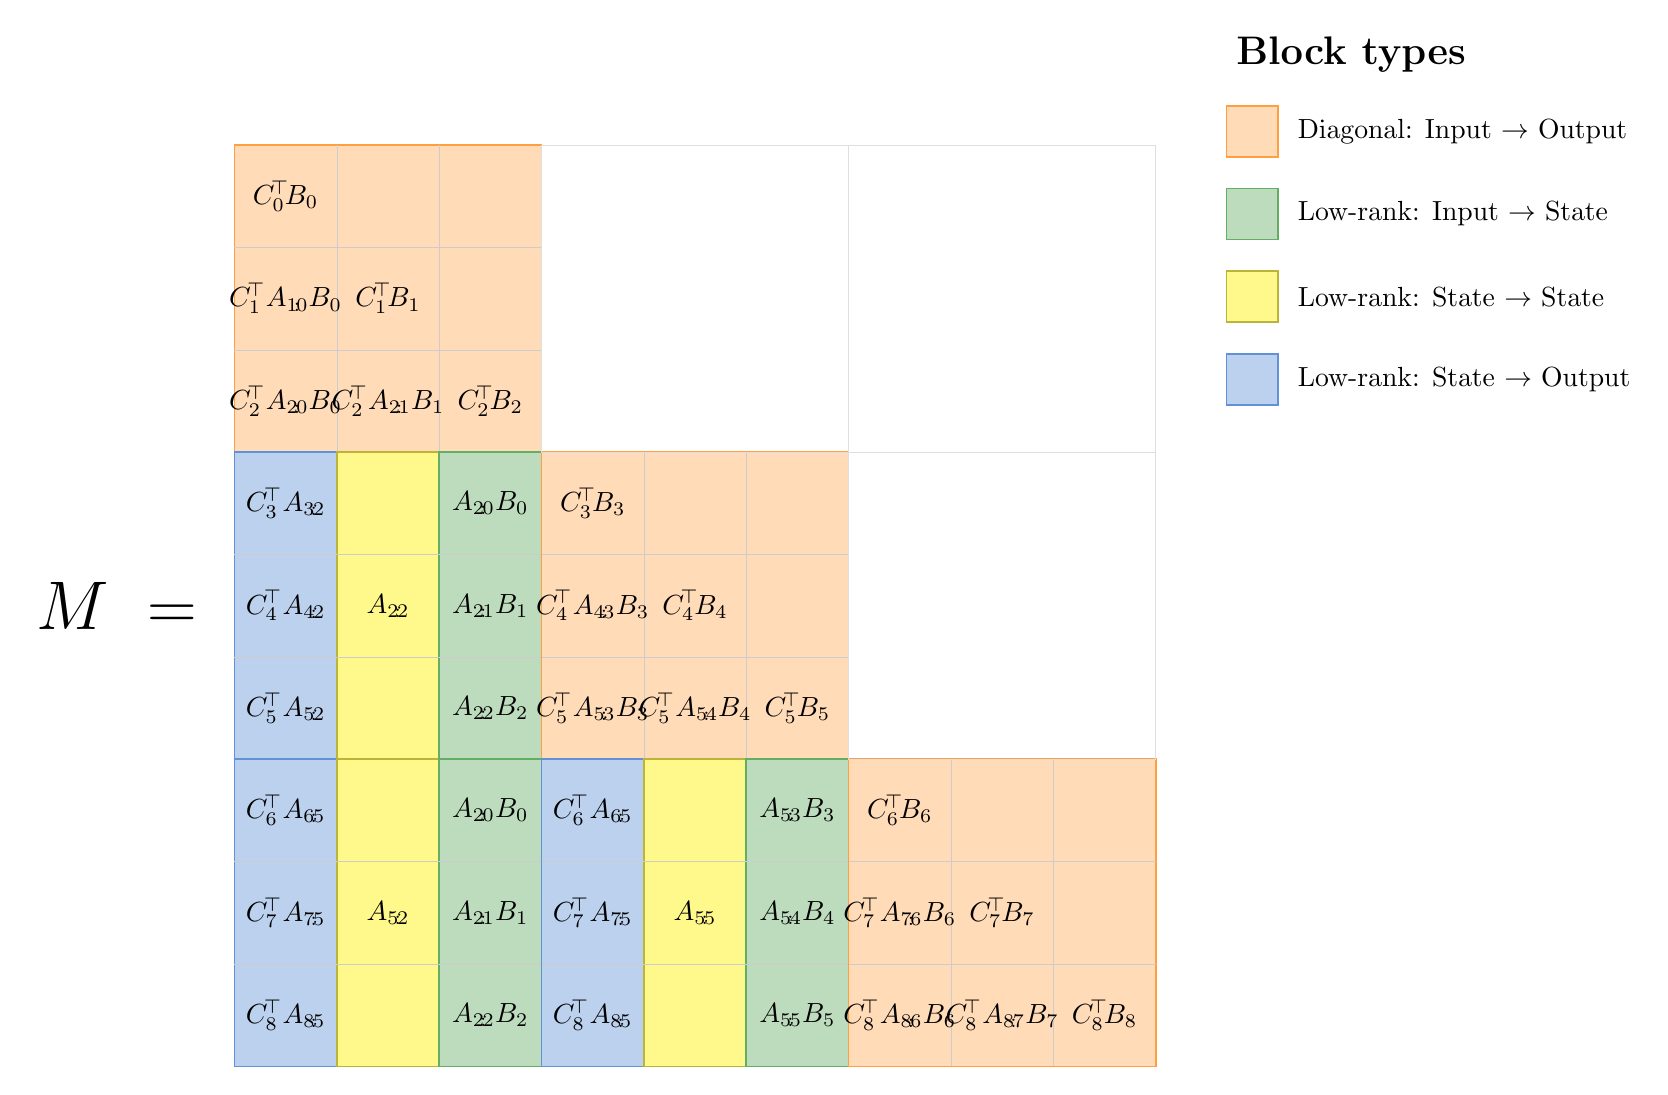
\begin{tikzpicture}[
    diagBlock/.style={fill=orange!28, draw=orange!75, semithick},
    isBlock/.style={fill=mambagreen!30, draw=mambagreen!70, semithick},
    ssBlock/.style={fill=yellow!45, draw=yellow!70!black, semithick},
    soBlock/.style={fill=mambablue!30, draw=mambablue!70, semithick},
    gridLine/.style={black!20, very thin},
    cellLab/.style={font=\normalsize, inner sep=1pt},
  ]

    %% =================== M matrix with explicit entries ===================
    \def\cw{1.30}     % sub-cell width
    \def\chw{3.90}    % chunk width = 3*cw

    % --- "M =" label on the left of the matrix ---
    \node[font=\Huge, anchor=east] at (-0.35, -1.5*\chw) {$M \;=$};

    % --- Diagonal chunk (0,0): rows/cols 0-2 ---
    \begin{scope}[shift={(0,0)}]
      \draw[diagBlock] (0,0) rectangle (\chw, -\chw);
      \foreach \k in {1,2} {
        \draw[gridLine] (\k*\cw, 0) -- (\k*\cw, -\chw);
        \draw[gridLine] (0, -\k*\cw) -- (\chw, -\k*\cw);
      }
      \node[cellLab] at (0.5*\cw, -0.5*\cw) {$C_0^{\!\top}\! B_0$};
      \node[cellLab] at (0.5*\cw, -1.5*\cw) {$C_1^{\!\top} A_{1\!:\!0} B_0$};
      \node[cellLab] at (1.5*\cw, -1.5*\cw) {$C_1^{\!\top}\! B_1$};
      \node[cellLab] at (0.5*\cw, -2.5*\cw) {$C_2^{\!\top} A_{2\!:\!0} B_0$};
      \node[cellLab] at (1.5*\cw, -2.5*\cw) {$C_2^{\!\top} A_{2\!:\!1} B_1$};
      \node[cellLab] at (2.5*\cw, -2.5*\cw) {$C_2^{\!\top}\! B_2$};
    \end{scope}

    % --- Off-diagonal chunk (1,0): rows 3-5, cols 0-2 ---
    \begin{scope}[shift={(0, -\chw)}]
      \draw[soBlock] (0, 0)       rectangle (\cw, -\chw);
      \draw[ssBlock] (\cw, 0)     rectangle (2*\cw, -\chw);
      \draw[isBlock] (2*\cw, 0)   rectangle (\chw, -\chw);
      \foreach \k in {1,2} {
        \draw[gridLine] (0, -\k*\cw) -- (\chw, -\k*\cw);
      }
      % Blue (C^T propagated to end of input chunk)
      \node[cellLab] at (0.5*\cw, -0.5*\cw) {$C_3^{\!\top} A_{3\!:\!2}$};
      \node[cellLab] at (0.5*\cw, -1.5*\cw) {$C_4^{\!\top} A_{4\!:\!2}$};
      \node[cellLab] at (0.5*\cw, -2.5*\cw) {$C_5^{\!\top} A_{5\!:\!2}$};
      % Yellow (inter-chunk A)
      \node[cellLab] at (1.5*\cw, -1.5*\cw) {$A_{2\!:\!2}$};
      % Green (A within input chunk * B)
      \node[cellLab] at (2.5*\cw, -0.5*\cw) {$A_{2\!:\!0} B_0$};
      \node[cellLab] at (2.5*\cw, -1.5*\cw) {$A_{2\!:\!1} B_1$};
      \node[cellLab] at (2.5*\cw, -2.5*\cw) {$A_{2\!:\!2} B_2$};
    \end{scope}

    % --- Diagonal chunk (1,1): rows/cols 3-5 ---
    \begin{scope}[shift={(\chw, -\chw)}]
      \draw[diagBlock] (0,0) rectangle (\chw, -\chw);
      \foreach \k in {1,2} {
        \draw[gridLine] (\k*\cw, 0) -- (\k*\cw, -\chw);
        \draw[gridLine] (0, -\k*\cw) -- (\chw, -\k*\cw);
      }
      \node[cellLab] at (0.5*\cw, -0.5*\cw) {$C_3^{\!\top}\! B_3$};
      \node[cellLab] at (0.5*\cw, -1.5*\cw) {$C_4^{\!\top} A_{4\!:\!3} B_3$};
      \node[cellLab] at (1.5*\cw, -1.5*\cw) {$C_4^{\!\top}\! B_4$};
      \node[cellLab] at (0.5*\cw, -2.5*\cw) {$C_5^{\!\top} A_{5\!:\!3} B_3$};
      \node[cellLab] at (1.5*\cw, -2.5*\cw) {$C_5^{\!\top} A_{5\!:\!4} B_4$};
      \node[cellLab] at (2.5*\cw, -2.5*\cw) {$C_5^{\!\top}\! B_5$};
    \end{scope}

    % --- Off-diagonal chunk (2,0): rows 6-8, cols 0-2 ---
    \begin{scope}[shift={(0, -2*\chw)}]
      \draw[soBlock] (0, 0)       rectangle (\cw, -\chw);
      \draw[ssBlock] (\cw, 0)     rectangle (2*\cw, -\chw);
      \draw[isBlock] (2*\cw, 0)   rectangle (\chw, -\chw);
      \foreach \k in {1,2} {
        \draw[gridLine] (0, -\k*\cw) -- (\chw, -\k*\cw);
      }
      \node[cellLab] at (0.5*\cw, -0.5*\cw) {$C_6^{\!\top} A_{6\!:\!5}$};
      \node[cellLab] at (0.5*\cw, -1.5*\cw) {$C_7^{\!\top} A_{7\!:\!5}$};
      \node[cellLab] at (0.5*\cw, -2.5*\cw) {$C_8^{\!\top} A_{8\!:\!5}$};
      \node[cellLab] at (1.5*\cw, -1.5*\cw) {$A_{5\!:\!2}$};
      \node[cellLab] at (2.5*\cw, -0.5*\cw) {$A_{2\!:\!0} B_0$};
      \node[cellLab] at (2.5*\cw, -1.5*\cw) {$A_{2\!:\!1} B_1$};
      \node[cellLab] at (2.5*\cw, -2.5*\cw) {$A_{2\!:\!2} B_2$};
    \end{scope}

    % --- Off-diagonal chunk (2,1): rows 6-8, cols 3-5 ---
    \begin{scope}[shift={(\chw, -2*\chw)}]
      \draw[soBlock] (0, 0)       rectangle (\cw, -\chw);
      \draw[ssBlock] (\cw, 0)     rectangle (2*\cw, -\chw);
      \draw[isBlock] (2*\cw, 0)   rectangle (\chw, -\chw);
      \foreach \k in {1,2} {
        \draw[gridLine] (0, -\k*\cw) -- (\chw, -\k*\cw);
      }
      \node[cellLab] at (0.5*\cw, -0.5*\cw) {$C_6^{\!\top} A_{6\!:\!5}$};
      \node[cellLab] at (0.5*\cw, -1.5*\cw) {$C_7^{\!\top} A_{7\!:\!5}$};
      \node[cellLab] at (0.5*\cw, -2.5*\cw) {$C_8^{\!\top} A_{8\!:\!5}$};
      \node[cellLab] at (1.5*\cw, -1.5*\cw) {$A_{5\!:\!5}$};
      \node[cellLab] at (2.5*\cw, -0.5*\cw) {$A_{5\!:\!3} B_3$};
      \node[cellLab] at (2.5*\cw, -1.5*\cw) {$A_{5\!:\!4} B_4$};
      \node[cellLab] at (2.5*\cw, -2.5*\cw) {$A_{5\!:\!5} B_5$};
    \end{scope}

    % --- Diagonal chunk (2,2): rows/cols 6-8 ---
    \begin{scope}[shift={(2*\chw, -2*\chw)}]
      \draw[diagBlock] (0,0) rectangle (\chw, -\chw);
      \foreach \k in {1,2} {
        \draw[gridLine] (\k*\cw, 0) -- (\k*\cw, -\chw);
        \draw[gridLine] (0, -\k*\cw) -- (\chw, -\k*\cw);
      }
      \node[cellLab] at (0.5*\cw, -0.5*\cw) {$C_6^{\!\top}\! B_6$};
      \node[cellLab] at (0.5*\cw, -1.5*\cw) {$C_7^{\!\top} A_{7\!:\!6} B_6$};
      \node[cellLab] at (1.5*\cw, -1.5*\cw) {$C_7^{\!\top}\! B_7$};
      \node[cellLab] at (0.5*\cw, -2.5*\cw) {$C_8^{\!\top} A_{8\!:\!6} B_6$};
      \node[cellLab] at (1.5*\cw, -2.5*\cw) {$C_8^{\!\top} A_{8\!:\!7} B_7$};
      \node[cellLab] at (2.5*\cw, -2.5*\cw) {$C_8^{\!\top}\! B_8$};
    \end{scope}

    % Above-diagonal (empty) chunk outlines
    \foreach \i/\j in {0/1, 0/2, 1/2} {
      \draw[gray!25, thin] ({\j*\chw}, {-\i*\chw})
                           rectangle ({(\j+1)*\chw}, {-(\i+1)*\chw});
    }
    %% =================== Legend (right of matrix) ===================
    \begin{scope}[shift={({3*\chw + 0.9}, -0.2)}]
      \node[font=\Large\bfseries, anchor=south west] at (0, 1.0)
        {Block types};
      \def\lh{-1.05}
      \draw[diagBlock] (0, {0.70+0*\lh}) rectangle (0.65, {0.05+0*\lh});
      \draw[isBlock]   (0, {0.70+1*\lh}) rectangle (0.65, {0.05+1*\lh});
      \draw[ssBlock]   (0, {0.70+2*\lh}) rectangle (0.65, {0.05+2*\lh});
      \draw[soBlock]   (0, {0.70+3*\lh}) rectangle (0.65, {0.05+3*\lh});
      \node[font=\normalsize, anchor=west] at (0.78, {0.375+0*\lh}) {Diagonal: Input $\to$ Output};
      \node[font=\normalsize, anchor=west] at (0.78, {0.375+1*\lh}) {Low-rank: Input $\to$ State};
      \node[font=\normalsize, anchor=west] at (0.78, {0.375+2*\lh}) {Low-rank: State $\to$ State};
      \node[font=\normalsize, anchor=west] at (0.78, {0.375+3*\lh}) {Low-rank: State $\to$ Output};
    \end{scope}

  \end{tikzpicture}
  }
  \end{center}
\end{frame}

% -----------------------------------------------------------------------
\begin{frame}{Chunked SSD: Conceptual Walkthrough}

  \textbf{Idea.} Cut the sequence into $Q$ chunks of size $C$, and exploit two facts:
  \begin{itemize}
    \item \emph{Inside} a chunk: a small $C{\times}C$ matmul handles all in-chunk dependencies.
    \item \emph{Across} chunks: each off-diagonal chunk-block of $M$ is rank $N$, so it can be summarized by a single state vector of size $N$. Only $Q \ll T$ such states are needed.
  \end{itemize}

  \vspace{0.4em}
  \textbf{The four pieces:}
  \begin{description}\itemsep1pt
    \item[\textcolor{orange!75!black}{$\blacksquare$ Diagonal}\ (intra-chunk Input$\to$Output).]
      For chunk $k$, compute the local SSM output via one small matmul on the $C{\times}C$ diagonal block $(L_k \circ C_k B_k^{\!\top})\,X_k$.
    \item[\textcolor{mambagreen!70!black}{$\blacksquare$ Input$\to$State}\ (end-of-chunk summary).]
      For chunk $k$, integrate inputs up to the chunk's right edge to get a single state vector $h_k^{\text{end}}\in\R^{N\times P}$.
    \item[\textcolor{yellow!60!black}{$\blacksquare$ State$\to$State}\ (inter-chunk recurrence).]
      Sequentially carry the chunk-final states: $H_{k+1} = a^{(k)}_{\text{cum}}\, H_k + h_k^{\text{end}}$. Only $Q$ steps.
    \item[\textcolor{mambablue!75!black}{$\blacksquare$ State$\to$Output}\ (spread incoming state).]
      For chunk $k$, broadcast the incoming state $H_k$ onto the chunk's outputs by another small matmul.
  \end{description}

  \vspace{0.3em}
  Then $Y = Y_{\text{intra}} + Y_{\text{inter}}$. Three of the four pieces are \emph{parallel-over-chunks matmuls} that hit tensor cores; only the yellow piece is sequential, and it has only $Q$ steps.
\end{frame}

% -----------------------------------------------------------------------
\begin{frame}{Chunked SSD: Algorithm}
  \begin{center}
  \footnotesize
  \begin{algorithm}[H]
    \caption{Chunked SSD (scalar $A_t = a_t$)}
    \KwIn{$X \in \R^{T \times P}$, $a \in \R^T$, $B, C \in \R^{T \times N}$; chunk size $C$, $Q = T/C$}
    \KwOut{$Y \in \R^{T \times P}$}
    \tcc{$a^\times_{i:j} := a_i\, a_{i-1}\cdots a_{j+1}$;\, $s_k = kC$,\, $e_k = (k{+}1)C - 1$}
    \BlankLine
    $\textcolor{orange!75!black}{\blacksquare}\;\; Y_{\text{intra}}^{(k)} \gets (L_k \circ C_k B_k^{\!\top})\, X_k$ \tcp*{\textbf{parallel} over chunks $k$: $Q$ independent $C{\times}C$ matmuls}
    $\textcolor{mambagreen!70!black}{\blacksquare}\;\; h_k^{\text{end}} \gets \sum_{t \in \text{chunk } k} a^\times_{e_k:t}\, B_t\, X_t$ \tcp*{\textbf{parallel} over $k$: one einsum, $Q$ states $\in \R^{N\times P}$}
    $\textcolor{yellow!60!black}{\blacksquare}\;\; L^{\!\times}[k,j] \gets a^\times_{e_{k-1}:e_j}\;\,(j < k)$ \tcp*{cross-chunk decay: \textbf{parallel scan} on $\log a$ ($O(\log Q)$ depth)}
    $\textcolor{yellow!60!black}{\blacksquare}\;\; H \gets L^{\!\times}\, h^{\text{end}}$ \tcp*{inter-chunk recurrence: one $Q{\times}Q$ matmul}
    $\textcolor{mambablue!75!black}{\blacksquare}\;\; Y_{\text{inter}}^{(k)}[i] \gets \bigl(a^\times_{i:s_k - 1}\, C_i\bigr)^{\!\top}\, H_k$ \tcp*{\textbf{parallel} over $k$: one einsum}
    \Return $Y \gets Y_{\text{intra}} + Y_{\text{inter}}$\;
  \end{algorithm}
  \end{center}

  \vspace{0.4em}
  \begin{itemize}\itemsep1pt
    \item \textbf{Parallel over chunks} (independent across $k$): orange, green, blue. Each is a single (ein)sum/matmul that hits tensor cores.
    \item \textbf{Sequential across chunks}: yellow only. The chunk-to-chunk dependency is the cumulative sum on $\log a$, which runs as a parallel scan in $O(\log Q)$ depth; the apply-to-states step is then a single $Q{\times}Q$ matmul.
    \item Total cost: $O(TCN + TCP)$.
  \end{itemize}
\end{frame}

% -----------------------------------------------------------------------
\begin{frame}{From $L$ to $L^\times$: Subsampling at Chunk Endpoints}

  Recall $L \in \R^{T \times T}$ with $L[i,j] = a^\times_{i:j}$ for $i \ge j$. $L^\times$ is the $Q{\times}Q$ matrix obtained by reading off $L$ at the chunk-end positions $e_q := (q{+}1)C - 1$:
  \[
    L^\times[k, j] \;=\; L\bigl[e_{k-1},\, e_j\bigr] \quad (j < k).
  \]

  \vspace{0.3em}
  \begin{center}
  \begin{tikzpicture}[scale=0.78]
    \def\cs{0.42}

    %% ============ L matrix (9x9), T=9, C=3, Q=3 ============
    % Lower triangle gray fill
    \foreach \r in {0,...,8} {
      \foreach \c in {0,...,8} {
        \pgfmathtruncatemacro{\below}{\c <= \r ? 1 : 0}
        \ifnum\below=1
          \fill[black!5] ({\c*\cs}, {-\r*\cs}) rectangle ({(\c+1)*\cs}, {-(\r+1)*\cs});
        \fi
      }
    }
    % Diagonal chunk orange tint (lower triangle within chunk)
    \foreach \k in {0,1,2} {
      \foreach \r in {0,1,2} {
        \foreach \c in {0,1,2} {
          \pgfmathtruncatemacro{\below}{\c <= \r ? 1 : 0}
          \ifnum\below=1
            \fill[orange!22] ({(\k*3+\c)*\cs}, {-(\k*3+\r)*\cs}) rectangle
                             ({(\k*3+\c+1)*\cs}, {-(\k*3+\r+1)*\cs});
          \fi
        }
      }
    }
    % Yellow highlight for chunk-end positions
    \foreach \row/\col in {2/2, 5/2, 5/5, 8/2, 8/5, 8/8} {
      \fill[yellow!60] ({\col*\cs}, {-\row*\cs}) rectangle ({(\col+1)*\cs}, {-(\row+1)*\cs});
    }
    % Thin grid
    \foreach \k in {0,...,9} {
      \draw[black!25, very thin] ({\k*\cs}, 0) -- ({\k*\cs}, {-9*\cs});
      \draw[black!25, very thin] (0, {-\k*\cs}) -- ({9*\cs}, {-\k*\cs});
    }
    % Thick chunk boundaries
    \foreach \k in {0,3,6,9} {
      \draw[thick] ({\k*\cs}, 0) -- ({\k*\cs}, {-9*\cs});
      \draw[thick] (0, {-\k*\cs}) -- ({9*\cs}, {-\k*\cs});
    }
    % Chunk-end labels
    \foreach \k/\name in {0/{e_0}, 1/{e_1}, 2/{e_2}} {
      \node[font=\scriptsize, anchor=south] at ({(\k*3+2.5)*\cs}, {0.04}) {$\name$};
      \node[font=\scriptsize, anchor=east]  at ({-0.04}, {-(\k*3+2.5)*\cs}) {$\name$};
    }
    % "L =" label below the L matrix
    \node[font=\large, anchor=north] at ({4.5*\cs}, {-9*\cs - 0.30}) {$L$};

    %% ============ Arrow with single combined label above ============
    \draw[-Stealth, very thick]
      ({9.6*\cs}, {-4.5*\cs}) -- ({15.4*\cs}, {-4.5*\cs});
    \node[font=\scriptsize, anchor=south] at ({12.5*\cs}, {-4.5*\cs+0.10})
      {sample at $\{e_q\}$};

    %% ============ L^x matrix (3x3), shifted further right; cells 1.4x larger ============
    \begin{scope}[shift={({16.2*\cs}, {-3.0*\cs})}]
      \def\cls{0.588}  % L^x cell size = 1.4 * \cs
      % Yellow cells (lower triangular incl diagonal)
      \foreach \r in {0,1,2} {
        \foreach \c in {0,1,2} {
          \pgfmathtruncatemacro{\below}{\c <= \r ? 1 : 0}
          \ifnum\below=1
            \fill[yellow!60] ({\c*\cls}, {-\r*\cls}) rectangle
                             ({(\c+1)*\cls}, {-(\r+1)*\cls});
          \fi
        }
      }
      % Values
      \node at ({0.5*\cls}, {-0.5*\cls}) {\scriptsize $1$};
      \node at ({0.5*\cls}, {-1.5*\cls}) {\scriptsize $\beta_1$};
      \node at ({1.5*\cls}, {-1.5*\cls}) {\scriptsize $1$};
      \node at ({0.5*\cls}, {-2.5*\cls}) {\scriptsize $\beta_1\beta_2$};
      \node at ({1.5*\cls}, {-2.5*\cls}) {\scriptsize $\beta_2$};
      \node at ({2.5*\cls}, {-2.5*\cls}) {\scriptsize $1$};
      % Borders
      \foreach \k in {0,1,2,3} {
        \draw[thick] ({\k*\cls}, 0) -- ({\k*\cls}, {-3*\cls});
        \draw[thick] (0, {-\k*\cls}) -- ({3*\cls}, {-\k*\cls});
      }
      % Axis labels
      \foreach \k/\name in {0/{0}, 1/{1}, 2/{2}} {
        \node[font=\scriptsize, anchor=south] at ({(\k+0.5)*\cls}, {0.04}) {$j{=}\name$};
      }
      \foreach \k/\name in {0/{1}, 1/{2}, 2/{3}} {
        \node[font=\scriptsize, anchor=east] at ({-0.04}, {-(\k+0.5)*\cls}) {$k{=}\name$};
      }
      % "L^x =" label below the small matrix
      \node[font=\large, anchor=north] at ({1.5*\cls}, {-3*\cls - 0.30}) {$L^\times$};
    \end{scope}

  \end{tikzpicture}
  \end{center}

  \textbf{Efficient computation.}
  \begin{itemize}\itemsep1pt
    \item Per-chunk total decay $\beta_q := \prod_{t \in \text{chunk } q} a_t$: one parallel reduction inside each chunk, all chunks in parallel.
    \item Parallel scan of $\{\beta_q\}$ gives cumulative products $P_q := \beta_0\,\beta_1\cdots\beta_q$ in $O(\log Q)$ depth.
    \item Pairwise ratio fills the whole matrix: $L^\times[k,j] = P_{k-1}/P_j$, one broadcast over $(k, j)$ pairs.
  \end{itemize}
\end{frame}

% -----------------------------------------------------------------------
\begin{frame}{Equivalence to $Y = MX$: Setup and Intra-Chunk Part}

  \textbf{Goal.} Show the four-step algorithm produces $y_i = (MX)_i$, where
  $M[i,j] = C_i^{\!\top} a^\times_{i:j}\, B_j$ for $j \le i$.

  \vspace{0.4em}
  \textbf{Notation.} $k$ = chunk containing the output position $i$; $\ell < k$ ranges over the earlier chunks. Within chunk $m$, token indices run $j \in [s_m, e_m]$.

  \vspace{0.4em}
  \textbf{Key identity (semigroup property of the scalar accumulator).}
  For any split point $j \le m \le i$,
  \[
    a^\times_{i:j} \;=\; a^\times_{i:m}\;\cdot\;a^\times_{m:j}.
  \]
  The entire proof is a single application of this identity at two well-chosen split points.

  \vspace{0.4em}
  \textbf{Step 1 -- split the sum at the left chunk boundary $s_k$:}
  \[
    y_i \;=\; \underbrace{\sum_{j = s_k}^{i} C_i^{\!\top} a^\times_{i:j} B_j X_j}_{\text{same chunk}}
            \;+\; \underbrace{\sum_{\ell < k}\;\sum_{j \,\in\, \text{chunk}\,\ell} C_i^{\!\top} a^\times_{i:j} B_j X_j}_{\text{earlier chunks (next slide)}}.
  \]

  \vspace{0.3em}
  \textbf{Step 2 -- same chunk.} The first sum is the restriction of the SSM to positions $[s_k, e_k]$, which is exactly the matrix $(L_k \circ C_k B_k^{\!\top}) X_k$ evaluated at row $i - s_k$:
  \[
    \sum_{j = s_k}^{i} C_i^{\!\top} a^\times_{i:j} B_j X_j
    \;=\; Y_{\text{intra}}^{(k)}[i]
    \qquad {\color{orange!75!black}\blacksquare\;\text{(orange line in algorithm).}}
  \]

  \vspace{0.3em}
  The remaining work is to rewrite the \emph{earlier chunks} sum as $Y_{\text{inter}}^{(k)}[i]$. That is the next slide.
\end{frame}

% -----------------------------------------------------------------------
\begin{frame}{Equivalence to $Y = MX$: Inter-Chunk Part}

  \textbf{Picking up from the previous slide:} the earlier-chunks contribution to $y_i$ is
  \[
    \sum_{\ell < k}\;\sum_{j \,\in\, \text{chunk}\,\ell} C_i^{\!\top} a^\times_{i:j} B_j X_j.
  \]

  \vspace{0.3em}
  \textbf{Step 3 -- apply the key identity twice} at $m = e_{k-1} = s_k - 1$ and at $m = e_\ell$:
  \[
    a^\times_{i:j} \;=\; \underbrace{a^\times_{i:\,e_{k-1}}}_{\text{state}\,\to\,\text{output}}
                       \;\cdot\; \underbrace{a^\times_{e_{k-1}:\,e_\ell}}_{=\,L^\times[k,\ell]\;(\text{state}\,\to\,\text{state})}
                       \;\cdot\; \underbrace{a^\times_{e_\ell:\,j}}_{\text{input}\,\to\,\text{state}}
    \qquad (j \in \text{chunk}\,\ell,\;\ell < k).
  \]
  The three factors depend on disjoint variables ($i$ only; $\ell$ only; $j$ and $\ell$), so the triple sum factorises:
  \[
    \sum_{\ell<k}\sum_{j\,\in\,\text{chunk}\,\ell}\! C_i^{\!\top} a^\times_{i:j} B_j X_j
    \;=\; \bigl(a^\times_{i:e_{k-1}}\,C_i\bigr)^{\!\top}\!
          \underbrace{\sum_{\ell<k} L^\times[k,\ell]\,
            \underbrace{\Bigl[\sum_{j\,\in\,\text{chunk}\,\ell} a^\times_{e_\ell:j}\,B_j X_j\Bigr]}_{h_\ell^{\text{end}}\;{\color{mambagreen!70!black}\blacksquare}}
          }_{H_k\;{\color{yellow!60!black}\blacksquare}}
    \;=\; Y_{\text{inter}}^{(k)}[i]\;{\color{mambablue!75!black}\blacksquare}.
  \]
  Each underbrace is exactly one line of the algorithm (matching colour). Adding to Step 2 gives $y_i = Y_{\text{intra}}^{(k)}[i] + Y_{\text{inter}}^{(k)}[i]$. \hfill$\square$

\end{frame}

% -----------------------------------------------------------------------
\subsubsection{Reference PyTorch Implementation}

% -----------------------------------------------------------------------
\begin{frame}[fragile]{Reference Implementation: the \texttt{segsum} Helper}

    \begin{itemize}
        \item Source: \texttt{ssd\_minimal\_discrete} in the official Mamba-2 repo (\texttt{mamba\_ssm/modules/ssd\_minimal.py})
        \item Pedagogical implementation. True implementation is a Triton kernel.
    \end{itemize}

  \vspace{0.5em}
\begin{lstlisting}
def segsum(x):
    """exp(segsum(A)) produces a 1-SS matrix."""
    T = x.size(-1)
    x_cumsum  = torch.cumsum(x, dim=-1)
    x_segsum  = x_cumsum[..., :, None] - x_cumsum[..., None, :]
    mask      = torch.tril(torch.ones(T, T, device=x.device, dtype=bool))
    x_segsum  = x_segsum.masked_fill(~mask, -torch.inf)
    return x_segsum

# Call sites inside ssd_minimal_discrete:
#   within each chunk  -> builds L_k of shape (l, l)
L           = torch.exp(segsum(A))
#   across chunks      -> builds L^x of shape (Q+1, Q+1)
decay_chunk = torch.exp(segsum(F.pad(A_cumsum[..., -1], (1, 0))))
\end{lstlisting}

  \vspace{0.3em}
  \textbf{Construction.} The input \texttt{x} is the vector of \emph{log gates} $\log a_t$ along the last axis.
  \begin{itemize}\itemsep1pt
    \item \texttt{x\_cumsum[i]}\,$= \sum_{t \le i} \log a_t = \log \alpha_i$. A single \texttt{cumsum} call, $O(\log T)$ parallel depth.
    \item Pairwise difference \texttt{x\_cumsum[i] - x\_cumsum[j]} equals $\log \alpha_i - \log \alpha_j = \log a^\times_{i:j}$ for $i \ge j$. 
    \item \texttt{tril(\dots)} retains only $i \ge j$; the strict upper triangle is assigned $-\infty$ so that \texttt{exp(\dots)} maps it to $0$.
  \end{itemize}

  \vspace{0.2em}
  \textbf{Numerical stability.} For long sequences with $a_t < 1$, the direct product $\prod_t a_t$ underflows. Working with $\log a_t$ and \texttt{cumsum} keeps intermediate values in a stable range; \texttt{exp} is applied only at the end, where outputs are bounded by $1$.
\end{frame}

% -----------------------------------------------------------------------
% The next three slides show the same code body of ssd_minimal_discrete
% as three adjacent listings (setup / intra-chunk / end-of-chunk). Each
% slide colours the focused block via backgroundcolor while the other
% two stay neutral (mambagray!10).
% -----------------------------------------------------------------------
\begin{frame}[fragile]{Reference Implementation: Setup and Chunking}

\begin{lstlisting}[aboveskip=0pt,belowskip=0pt,frame=none,backgroundcolor=\color{mambablue!12}]
def ssd_minimal_discrete(X, A, B, C, block_len, initial_states=None):
    # X: (B, T, H, P),  A: (B, T, H),  B, C: (B, T, H, N)
    # Split time axis T = Q * block_len into Q chunks
    X, A, B, C = [rearrange(x, "b (c l) ... -> b c l ...", l=block_len)
                  for x in (X, A, B, C)]
    A         = rearrange(A, "b c l h -> b h c l")
    A_cumsum  = torch.cumsum(A, dim=-1)
\end{lstlisting}
\begin{lstlisting}[aboveskip=0pt,belowskip=0pt,frame=none,backgroundcolor=\color{mambagray!10}]

    # (1) Intra-chunk output  -- ORANGE diagonal blocks
    L      = torch.exp(segsum(A))
    Y_diag = torch.einsum("bclhn,bcshn,bhcls,bcshp->bclhp",
                          C, B, L, X)
\end{lstlisting}
\begin{lstlisting}[aboveskip=0pt,belowskip=0pt,frame=none,backgroundcolor=\color{mambagray!10}]

    # (2) End-of-chunk states -- GREEN  (input -> state)
    decay_states = torch.exp(A_cumsum[..., -1:] - A_cumsum)
    states       = torch.einsum("bclhn,bhcl,bclhp->bchpn",
                                B, decay_states, X)
\end{lstlisting}

  \vspace{0.3em}
  \textbf{Shape setup} (highlighted region).
  \begin{itemize}\itemsep1pt
    \item \texttt{rearrange("b (c l) ... -> b c l ...", l=block\_len)} factorises the time axis $T = Q \cdot C$, exposing the chunk index \texttt{c} and the within-chunk index \texttt{l}. The operation is a view; no data is copied.
    \item The subsequent \texttt{rearrange} on \texttt{A} moves the head axis next to the batch axis, producing layout \texttt{(B, H, Q, l)}. This makes the per-head, per-chunk operations that follow contiguous in memory.
    \item \texttt{A\_cumsum[b, h, c, l]}\,$= \sum_{t = s_c}^{s_c + l} \log a_t$. The \texttt{cumsum} is taken along \texttt{l} only, so each chunk carries an independent running log-product; the cross-chunk contribution is reconstructed later via \texttt{decay\_chunk}.
  \end{itemize}
\end{frame}

% -----------------------------------------------------------------------
\begin{frame}[fragile]{Reference Implementation: Intra-Chunk Output}

\begin{lstlisting}[aboveskip=0pt,belowskip=0pt,frame=none,backgroundcolor=\color{mambagray!10}]
def ssd_minimal_discrete(X, A, B, C, block_len, initial_states=None):
    # X: (B, T, H, P),  A: (B, T, H),  B, C: (B, T, H, N)
    # Split time axis T = Q * block_len into Q chunks
    X, A, B, C = [rearrange(x, "b (c l) ... -> b c l ...", l=block_len)
                  for x in (X, A, B, C)]
    A         = rearrange(A, "b c l h -> b h c l")
    A_cumsum  = torch.cumsum(A, dim=-1)
\end{lstlisting}
\begin{lstlisting}[aboveskip=0pt,belowskip=0pt,frame=none,backgroundcolor=\color{orange!18}]

    # (1) Intra-chunk output  -- ORANGE diagonal blocks
    L      = torch.exp(segsum(A))
    Y_diag = torch.einsum("bclhn,bcshn,bhcls,bcshp->bclhp",
                          C, B, L, X)
\end{lstlisting}
\begin{lstlisting}[aboveskip=0pt,belowskip=0pt,frame=none,backgroundcolor=\color{mambagray!10}]

    # (2) End-of-chunk states -- GREEN  (input -> state)
    decay_states = torch.exp(A_cumsum[..., -1:] - A_cumsum)
    states       = torch.einsum("bclhn,bhcl,bclhp->bchpn",
                                B, decay_states, X)
\end{lstlisting}

  \vspace{0.3em}
  \textbf{(1) Intra-chunk output} (highlighted region).
  \begin{itemize}\itemsep1pt
    \item \texttt{L = torch.exp(segsum(A))} produces, for every (batch, head, chunk), the lower-triangular $l \times l$ matrix $L_k$ from the proof, with entries $L_k[i,j] = a^\times_{s_k+i:\,s_k+j}$ for $i \ge j$.
    \item The einsum \texttt{"bclhn,bcshn,bhcls,bcshp->bclhp"} evaluates $(L_k \circ C_k B_k^{\!\top}) X_k$ for every (batch, head, chunk) simultaneously. The contracted index \texttt{n} produces the score $C_l^{\!\top} B_s$; the contracted index \texttt{s} (key position within the chunk) couples this score with the causal mask $L$ and the input $X$.
    \item The free indices \texttt{b,c,h,l,p} form the output shape, identical to the input layout.
  \end{itemize}
\end{frame}

% -----------------------------------------------------------------------
\begin{frame}[fragile]{Reference Implementation: End-of-Chunk States}

\begin{lstlisting}[aboveskip=0pt,belowskip=0pt,frame=none,backgroundcolor=\color{mambagray!10}]
def ssd_minimal_discrete(X, A, B, C, block_len, initial_states=None):
    # X: (B, T, H, P),  A: (B, T, H),  B, C: (B, T, H, N)
    # Split time axis T = Q * block_len into Q chunks
    X, A, B, C = [rearrange(x, "b (c l) ... -> b c l ...", l=block_len)
                  for x in (X, A, B, C)]
    A         = rearrange(A, "b c l h -> b h c l")
    A_cumsum  = torch.cumsum(A, dim=-1)
\end{lstlisting}
\begin{lstlisting}[aboveskip=0pt,belowskip=0pt,frame=none,backgroundcolor=\color{orange!15}]

    # (1) Intra-chunk output  -- ORANGE  (input -> output, diagonal blocks)
    L      = torch.exp(segsum(A))
    Y_diag = torch.einsum("bclhn,bcshn,bhcls,bcshp->bclhp",
                          C, B, L, X)
\end{lstlisting}
\begin{lstlisting}[aboveskip=0pt,belowskip=0pt,frame=none,backgroundcolor=\color{mambagreen!18}]

    # (2) End-of-chunk states -- GREEN  (input -> state)
    decay_states = torch.exp(A_cumsum[..., -1:] - A_cumsum)
    states       = torch.einsum("bclhn,bhcl,bclhp->bchpn",
                                B, decay_states, X)
\end{lstlisting}

  \vspace{0.3em}
  \textbf{(2) End-of-chunk states} (highlighted region).
  \begin{itemize}\itemsep1pt
    \item For token $t$ inside chunk $k$, the contribution to $h_k^{\text{end}}$ is weighted by $a^\times_{e_k : t} = \alpha_{e_k}/\alpha_t = \exp(\log\alpha_{e_k} - \log\alpha_t)$.
    \item \texttt{A\_cumsum} has shape \texttt{(B, H, Q, l)} with \texttt{A\_cumsum[..., t]} $= \log\alpha_t = \sum_{s \le t}\log a_s$ (running within-chunk log-decay).
%    \item \texttt{A\_cumsum[..., -1:]} selects the last within-chunk position, shape \texttt{(B, H, Q, 1)}: the total chunk log-decay $\log\alpha_{e_k}$. The slice \texttt{-1:} (not \texttt{-1}) keeps the trailing dimension so it broadcasts.
    \item \texttt{A\_cumsum[..., -1:] - A\_cumsum} broadcasts $(B,H,Q,1) - (B,H,Q,l) \to (B,H,Q,l)$, yielding $\log\alpha_{e_k} - \log\alpha_t$ for every (chunk, token). Taking \texttt{exp} gives \texttt{decay\_states[..., t]} $= a^\times_{e_k : t}$.
    \item The einsum \texttt{"bclhn,bhcl,bclhp->bchpn"} contracts the within-chunk time axis \texttt{l}, evaluating $h_k^{\text{end}} = \sum_{t \in \text{chunk}\,k} a^\times_{e_k:t}\,B_t\,X_t^{\!\top}$. The result has shape \texttt{(B, Q, H, P, N)}, i.e.\ one state in $\R^{N \times P}$ per (batch, head, chunk).
  \end{itemize}
\end{frame}

% -----------------------------------------------------------------------
\begin{frame}[fragile]{Reference Implementation: Inter-Chunk Recurrence and Output}

\begin{lstlisting}[aboveskip=0pt,belowskip=0pt,frame=none,backgroundcolor=\color{yellow!22}]
    # (3) Inter-chunk recurrence -- YELLOW  (state -> state)
    if initial_states is None:
        initial_states = torch.zeros_like(states[:, :1])
    states           = torch.cat([initial_states, states], dim=1)
    decay_chunk      = torch.exp(segsum(F.pad(A_cumsum[..., -1], (1, 0))))
    new_states       = torch.einsum("bhzc,bchpn->bzhpn", decay_chunk, states)
    states, final_state = new_states[:, :-1], new_states[:, -1]
\end{lstlisting}
\begin{lstlisting}[aboveskip=0pt,belowskip=0pt,frame=none,backgroundcolor=\color{mambablue!15}]

    # (4) State -> output -- BLUE  (state -> output)
    state_decay_out  = torch.exp(A_cumsum)                       # a^x_{i : s_k - 1}
    Y_off            = torch.einsum("bclhn,bchpn,bhcl->bclhp",
                                    C, states, state_decay_out)

    Y = rearrange(Y_diag + Y_off, "b c l h -> b (c l) h")
    return Y, final_state
\end{lstlisting}

  \vspace{0.3em}
  \textbf{(3) Inter-chunk recurrence.}
  \begin{itemize}\itemsep1pt
    \item \texttt{A\_cumsum[..., -1]} is one scalar per chunk: the total log-gate, $\sum_{t \in \text{chunk}\,k} \log a_t$. \texttt{F.pad(\dots, (1,0))} prepends a zero, reserving slot $0$ for the initial state.
    \item \texttt{segsum} of this $(Q{+}1)$-vector constructs the $(Q{+}1) \times (Q{+}1)$ matrix $L^\times$ across chunks: the second application of the 1-SS construction.
    \item The einsum \texttt{"bhzc,bchpn->bzhpn"} is a $Q{\times}Q$ matmul on the prepended \texttt{states} tensor; the recurrence $H_{k+1} = a^{\text{chunk}}_k H_k + h_k^{\text{end}}$ is evaluated as a single matmul. \texttt{final\_state} is returned so that callers may continue beyond the current window.
  \end{itemize}

  \vspace{0.2em}
  \textbf{(4) State $\to$ output.} \texttt{state\_decay\_out = exp(A\_cumsum)} is the within-chunk decay $a^\times_{i : s_k - 1}$ from the inherited state at $s_k - 1$ to position $i$. The einsum evaluates $Y_{\text{inter}}^{(k)}[i] = (a^\times_{i : s_k - 1}\, C_i)^{\!\top}\, H_k$ for every position.
\end{frame}

% -----------------------------------------------------------------------
\subsubsection{The Mamba-2 Architecture}

% -----------------------------------------------------------------------
\begin{frame}{Mamba-2 Block~\cite{dao2024mamba2}}
  \begin{columns}[T,onlytextwidth]
    \begin{column}{0.52\textwidth}
      \begin{center}
      \begin{tikzpicture}[
        op/.style={draw, thick, rounded corners=2pt, fill=gray!8,
                   minimum height=0.42cm, minimum width=1.35cm,
                   font=\tiny, align=center, inner sep=2pt},
        ssm/.style={draw, thick, rounded corners=3pt, fill=gray!8,
                    minimum height=0.55cm, minimum width=2.85cm,
                    font=\tiny\bfseries, align=center},
        silu/.style={draw, fill=black, text=white, rounded corners=3pt,
                     minimum height=0.30cm, minimum width=0.75cm,
                     font=\tiny, inner sep=1pt},
        siluwide/.style={draw, fill=black, text=white, rounded corners=3pt,
                         minimum height=0.30cm, minimum width=2.10cm,
                         font=\tiny, inner sep=1pt},
        mul/.style={draw, fill=black, text=white, rounded corners=3pt,
                    minimum height=0.30cm, minimum width=0.38cm,
                    font=\tiny, inner sep=1pt},
        cell/.style={draw=black!75, line width=0.3pt, minimum width=0.20cm,
                     minimum height=0.20cm, inner sep=0pt},
        arr/.style={-Stealth, semithick},
        scale=0.55, every node/.style={scale=0.55},
      ]
        \def\cellsz{0.21}
        \def\xX{-1.60}
        \def\xB{-0.80}
        \def\xCp{0.00}
        \def\xD{ 0.80}
        \def\xZ{ 1.60}
        \def\xC{ 0.00}
        \def\xMain{-0.40}

        % ====== Input vec ======
        \foreach \i/\c in {0/cellpinkA, 1/cellpinkB, 2/cellpinkC, 3/cellpinkD} {
          \node[cell, fill=\c] at (\xC-0.33+\i*\cellsz, 7.50) {};
        }
        \node[font=\scriptsize\bfseries, anchor=east] at (\xC-0.50, 7.50) {Input};

        % ====== Residual takeoff ======
        \draw[semithick] (\xC+0.40, 7.50) -- (2.95, 7.50) -- (2.95, -1.95);

        % ====== Dashed box ======
        \draw[dashed, thick, black!55, rounded corners=4pt]
          (-2.40, -1.45) rectangle (2.60, 6.95);

        % ====== Input arrow into block ======
        \draw[arr] (\xC, 7.35) -- (\xC, 6.65);

        % ====== Linear Projection trapezoid (1 -> 5) ======
        \draw[thick, fill=gray!3]
          (\xC-0.40, 6.65) -- (\xC+0.40, 6.65) --
          (2.00, 6.05) -- (-2.00, 6.05) -- cycle;
        \node[font=\tiny\bfseries] at (\xC, 6.35) {Linear Projection};

        % ====== Wide pink vec ======
        \foreach \i in {0,...,12} {
          \pgfmathtruncatemacro{\colidx}{mod(\i*3+1,5)}
          \ifnum\colidx=0 \node[cell, fill=cellpinkB] at ({-1.92+\i*0.32}, 5.85) {}; \fi
          \ifnum\colidx=1 \node[cell, fill=cellpinkA] at ({-1.92+\i*0.32}, 5.85) {}; \fi
          \ifnum\colidx=2 \node[cell, fill=cellpinkC] at ({-1.92+\i*0.32}, 5.85) {}; \fi
          \ifnum\colidx=3 \node[cell, fill=cellpinkD] at ({-1.92+\i*0.32}, 5.85) {}; \fi
          \ifnum\colidx=4 \node[cell, fill=cellpinkB] at ({-1.92+\i*0.32}, 5.85) {}; \fi
        }

        % ====== Section labels ======
        \node[font=\tiny] at (\xX, 5.55)  {$X$};
        \node[font=\tiny] at (\xB, 5.55)  {$B$};
        \node[font=\tiny] at (\xCp, 5.55) {$C$};
        \node[font=\tiny] at (\xD, 5.55)  {$\Delta$};
        \node[font=\tiny] at (\xZ, 5.55)  {$Z$};

        % ====== Arrows from sections ======
        % X, B, C: down to Conv1D top
        \draw[arr] (\xX,  5.35) -- (\xX,  5.00);
        \draw[arr] (\xB,  5.35) -- (\xB,  5.00);
        \draw[arr] (\xCp, 5.35) -- (\xCp, 5.00);
        % Δ: bypass Conv/SiLU, straight down to SSD top
        \draw[arr] (\xD,  5.35) -- (\xD,  3.10);
        % Z: bypass to SiLU(Z)
        \draw[arr] (\xZ,  5.35) -- (\xZ,  3.40);

        % ====== Conv1D (over X, B, C) ======
        \node[op, minimum width=2.15cm, minimum height=0.42cm]
             (conv) at ({(\xX+\xCp)/2}, 4.78) {Conv1D};

        % Arrows Conv -> SiLU
        \draw[arr] (\xX,  4.57) -- (\xX,  4.20);
        \draw[arr] (\xB,  4.57) -- (\xB,  4.20);
        \draw[arr] (\xCp, 4.57) -- (\xCp, 4.20);

        % ====== SiLU (over X, B, C) ======
        \node[siluwide] (siluL) at ({(\xX+\xCp)/2}, 4.02) {SiLU};

        % Arrows SiLU L -> SSD
        \draw[arr] (\xX,  3.85) -- (\xX,  3.10);
        \draw[arr] (\xB,  3.85) -- (\xB,  3.10);
        \draw[arr] (\xCp, 3.85) -- (\xCp, 3.10);

        % ====== SiLU (on Z) ======
        \node[silu] (siluZ) at (\xZ, 3.25) {SiLU};

        % ====== SSD Block ======
        \node[ssm] (ssd) at (\xMain, 2.82) {SSD Block};

        % SSD output to RMSNorm
        \draw[arr] (ssd.south) -- (\xMain, 2.10);

        % ====== RMSNorm ======
        \node[op, minimum width=1.30cm] (norm) at (\xMain, 1.88) {RMSNorm};

        % Norm to Multiply
        \draw[arr] (norm.south) -- (\xMain, 1.25);

        % ====== Multiply ======
        \node[mul] (mult) at (\xMain, 1.05) {$\times$};
        \draw[arr] (siluZ.south) -- (\xZ, 1.05) -- (mult.east);

        % Multiply down to blue vec
        \draw[arr] (mult.south) -- (\xMain, 0.45);

        % ====== Blue large vec ======
        \foreach \i/\c in {0/cellblueB, 1/cellblueA, 2/cellblueC, 3/cellblueA, 4/cellblueD, 5/cellblueC, 6/cellblueA} {
          \node[cell, fill=\c] at (\xMain-0.66+\i*\cellsz, 0.28) {};
        }
        \draw[arr] (\xMain, 0.15) -- (\xMain, -0.30);

        % ====== Output projection ======
        \draw[thick, fill=gray!3]
          (\xMain-0.85, -0.30) -- (\xMain+0.85, -0.30) --
          (\xMain+0.40, -0.90) -- (\xMain-0.40, -0.90) -- cycle;
        \node[font=\tiny\bfseries] at (\xMain, -0.60) {Projection};

        % ====== Small blue vec ======
        \foreach \i/\c in {0/cellblueA, 1/cellblueC, 2/cellblueB, 3/cellblueD} {
          \node[cell, fill=\c] at (\xMain-0.33+\i*\cellsz, -1.18) {};
        }

        % ====== Arrow out of box to + ======
        \draw[arr] (\xMain, -1.30) -- (\xMain, -1.95) -- (\xC-0.20, -1.95);

        % ====== + (residual) ======
        \node[mul] (resadd) at (\xC, -1.95) {$+$};
        \draw[arr] (2.95, -1.95) -- (resadd.east);

        % ====== Output vec ======
        \foreach \i/\c in {0/cellpurpA, 1/cellpurpC, 2/cellpurpB, 3/cellpurpD} {
          \node[cell, fill=\c] at (\xC-0.33+\i*\cellsz, -2.75) {};
        }
        \draw[arr] (resadd.south) -- (\xC, -2.60);
        \node[font=\scriptsize\bfseries, anchor=east] at (\xC-0.50, -2.75) {Output};
      \end{tikzpicture}
      \end{center}
    \end{column}
    \begin{column}{0.48\textwidth}
      \small
      \textbf{Dimensions:}
      \begin{itemize}
        \item $L$: sequence length
        \item $D = d_{\text{model}}$: model dimension
        \item $H$: number of heads
        \item $P$: head dim. ($64$--$128$, vs.\ $1$ in Mamba-1)
        \item $N$: SSM state size ($64$--$256{+}$, vs.\ $16$)
      \end{itemize}

      \vspace{0.3em}
      \textbf{Linear Projection:} a single \texttt{in\_proj} produces $[Z, X, B, C, \Delta]$ \emph{in parallel} (Mamba-1 routes $\Delta, B, C$ through a separate \texttt{Linear} on $\mathrm{SiLU}(\mathrm{Conv}(X))$).

      \vspace{0.3em}
      \textbf{SSD Block:}
      \begin{itemize}
        \item Scalar $A$ (one per head), not diagonal per channel
        \item Chunked algorithm: matmul-based, hits tensor cores
        \item \alert{$2$--$8\times$} faster training than Mamba-1
      \end{itemize}

      \vspace{0.3em}
      \textbf{Gate:} $Y \gets \mathrm{RMSNorm}(Y_{\text{SSD}}) \odot \mathrm{SiLU}(Z)$ (Mamba-2 keeps the norm \emph{inside} the block).
    \end{column}
  \end{columns}
\end{frame}

% -----------------------------------------------------------------------
\subsubsection{Comparison and Results}

% -----------------------------------------------------------------------
\begin{frame}{Mamba-2 vs.\ Mamba-1: Key Differences}

  \begin{center}
  \begin{tabular}{lll}
    \toprule
    & \textbf{Mamba-1} & \textbf{Mamba-2} \\
    \midrule
    Structure on $A$    & Diagonal         & Scalar-times-identity \\
    Head dimension $P$  & 1 (per channel)  & 64--128 \\
    State dimension $N$ & 16               & 64--256+ \\
    $(A,B,C)$ generation & Sequential       & Parallel with $X$ \\
    Training algorithm  & Selective scan   & Chunked SSD (matmuls) \\
    Tensor parallelism  & Harder           & Native support \\
    Training speed      & Slower           & \textbf{2--8$\times$ faster} \\
    Inference           & Faster (smaller $N$) & Slightly slower \\
    \bottomrule
  \end{tabular}
  \end{center}

\end{frame}

% -----------------------------------------------------------------------
\begin{frame}{Summary: State Space Models and Mamba}

  \begin{enumerate}
    \item \textbf{State Space Models}: Linear systems discretized from continuous time; dual recurrent/convolutional view enables parallel training for LTI models
    \item \textbf{Mamba-1}: Makes SSM parameters \emph{input-dependent} (selective); hardware-aware scan keeps computation in SRAM; matches Transformer quality with linear-time inference
    \item \textbf{State Space Duality}: Scalar-structured SSMs and causal linear attention are the \emph{same} model viewed differently
    \item \textbf{Mamba-2}: Chunked SSD algorithm: $O(TCN)$ compute, constant inference state, full matmul utilization; 2--8$\times$ faster training than Mamba-1
  \end{enumerate}

  \vspace{0.5em}
  \begin{block}{References}
    \cite{gu2022s4} \quad \cite{gu2024mamba} \quad \cite{dao2024mamba2}
  \end{block}
\end{frame}

